\documentclass[]{article}
\usepackage{lmodern}
\usepackage{amssymb,amsmath}
\usepackage{ifxetex,ifluatex}
\usepackage{fixltx2e} % provides \textsubscript
\ifnum 0\ifxetex 1\fi\ifluatex 1\fi=0 % if pdftex
  \usepackage[T1]{fontenc}
  \usepackage[utf8]{inputenc}
\else % if luatex or xelatex
  \ifxetex
    \usepackage{mathspec}
  \else
    \usepackage{fontspec}
  \fi
  \defaultfontfeatures{Ligatures=TeX,Scale=MatchLowercase}
\fi
% use upquote if available, for straight quotes in verbatim environments
\IfFileExists{upquote.sty}{\usepackage{upquote}}{}
% use microtype if available
\IfFileExists{microtype.sty}{%
\usepackage{microtype}
\UseMicrotypeSet[protrusion]{basicmath} % disable protrusion for tt fonts
}{}
\usepackage[margin=1in]{geometry}
\usepackage{hyperref}
\hypersetup{unicode=true,
            pdftitle={Analysis of},
            pdfborder={0 0 0},
            breaklinks=true}
\urlstyle{same}  % don't use monospace font for urls
\usepackage{color}
\usepackage{fancyvrb}
\newcommand{\VerbBar}{|}
\newcommand{\VERB}{\Verb[commandchars=\\\{\}]}
\DefineVerbatimEnvironment{Highlighting}{Verbatim}{commandchars=\\\{\}}
% Add ',fontsize=\small' for more characters per line
\usepackage{framed}
\definecolor{shadecolor}{RGB}{248,248,248}
\newenvironment{Shaded}{\begin{snugshade}}{\end{snugshade}}
\newcommand{\KeywordTok}[1]{\textcolor[rgb]{0.13,0.29,0.53}{\textbf{#1}}}
\newcommand{\DataTypeTok}[1]{\textcolor[rgb]{0.13,0.29,0.53}{#1}}
\newcommand{\DecValTok}[1]{\textcolor[rgb]{0.00,0.00,0.81}{#1}}
\newcommand{\BaseNTok}[1]{\textcolor[rgb]{0.00,0.00,0.81}{#1}}
\newcommand{\FloatTok}[1]{\textcolor[rgb]{0.00,0.00,0.81}{#1}}
\newcommand{\ConstantTok}[1]{\textcolor[rgb]{0.00,0.00,0.00}{#1}}
\newcommand{\CharTok}[1]{\textcolor[rgb]{0.31,0.60,0.02}{#1}}
\newcommand{\SpecialCharTok}[1]{\textcolor[rgb]{0.00,0.00,0.00}{#1}}
\newcommand{\StringTok}[1]{\textcolor[rgb]{0.31,0.60,0.02}{#1}}
\newcommand{\VerbatimStringTok}[1]{\textcolor[rgb]{0.31,0.60,0.02}{#1}}
\newcommand{\SpecialStringTok}[1]{\textcolor[rgb]{0.31,0.60,0.02}{#1}}
\newcommand{\ImportTok}[1]{#1}
\newcommand{\CommentTok}[1]{\textcolor[rgb]{0.56,0.35,0.01}{\textit{#1}}}
\newcommand{\DocumentationTok}[1]{\textcolor[rgb]{0.56,0.35,0.01}{\textbf{\textit{#1}}}}
\newcommand{\AnnotationTok}[1]{\textcolor[rgb]{0.56,0.35,0.01}{\textbf{\textit{#1}}}}
\newcommand{\CommentVarTok}[1]{\textcolor[rgb]{0.56,0.35,0.01}{\textbf{\textit{#1}}}}
\newcommand{\OtherTok}[1]{\textcolor[rgb]{0.56,0.35,0.01}{#1}}
\newcommand{\FunctionTok}[1]{\textcolor[rgb]{0.00,0.00,0.00}{#1}}
\newcommand{\VariableTok}[1]{\textcolor[rgb]{0.00,0.00,0.00}{#1}}
\newcommand{\ControlFlowTok}[1]{\textcolor[rgb]{0.13,0.29,0.53}{\textbf{#1}}}
\newcommand{\OperatorTok}[1]{\textcolor[rgb]{0.81,0.36,0.00}{\textbf{#1}}}
\newcommand{\BuiltInTok}[1]{#1}
\newcommand{\ExtensionTok}[1]{#1}
\newcommand{\PreprocessorTok}[1]{\textcolor[rgb]{0.56,0.35,0.01}{\textit{#1}}}
\newcommand{\AttributeTok}[1]{\textcolor[rgb]{0.77,0.63,0.00}{#1}}
\newcommand{\RegionMarkerTok}[1]{#1}
\newcommand{\InformationTok}[1]{\textcolor[rgb]{0.56,0.35,0.01}{\textbf{\textit{#1}}}}
\newcommand{\WarningTok}[1]{\textcolor[rgb]{0.56,0.35,0.01}{\textbf{\textit{#1}}}}
\newcommand{\AlertTok}[1]{\textcolor[rgb]{0.94,0.16,0.16}{#1}}
\newcommand{\ErrorTok}[1]{\textcolor[rgb]{0.64,0.00,0.00}{\textbf{#1}}}
\newcommand{\NormalTok}[1]{#1}
\usepackage{longtable,booktabs}
\usepackage{graphicx,grffile}
\makeatletter
\def\maxwidth{\ifdim\Gin@nat@width>\linewidth\linewidth\else\Gin@nat@width\fi}
\def\maxheight{\ifdim\Gin@nat@height>\textheight\textheight\else\Gin@nat@height\fi}
\makeatother
% Scale images if necessary, so that they will not overflow the page
% margins by default, and it is still possible to overwrite the defaults
% using explicit options in \includegraphics[width, height, ...]{}
\setkeys{Gin}{width=\maxwidth,height=\maxheight,keepaspectratio}
\IfFileExists{parskip.sty}{%
\usepackage{parskip}
}{% else
\setlength{\parindent}{0pt}
\setlength{\parskip}{6pt plus 2pt minus 1pt}
}
\setlength{\emergencystretch}{3em}  % prevent overfull lines
\providecommand{\tightlist}{%
  \setlength{\itemsep}{0pt}\setlength{\parskip}{0pt}}
\setcounter{secnumdepth}{0}
% Redefines (sub)paragraphs to behave more like sections
\ifx\paragraph\undefined\else
\let\oldparagraph\paragraph
\renewcommand{\paragraph}[1]{\oldparagraph{#1}\mbox{}}
\fi
\ifx\subparagraph\undefined\else
\let\oldsubparagraph\subparagraph
\renewcommand{\subparagraph}[1]{\oldsubparagraph{#1}\mbox{}}
\fi

%%% Use protect on footnotes to avoid problems with footnotes in titles
\let\rmarkdownfootnote\footnote%
\def\footnote{\protect\rmarkdownfootnote}

%%% Change title format to be more compact
\usepackage{titling}

% Create subtitle command for use in maketitle
\newcommand{\subtitle}[1]{
  \posttitle{
    \begin{center}\large#1\end{center}
    }
}

\setlength{\droptitle}{-2em}

  \title{Analysis of}
    \pretitle{\vspace{\droptitle}\centering\huge}
  \posttitle{\par}
    \author{}
    \preauthor{}\postauthor{}
      \predate{\centering\large\emph}
  \postdate{\par}
    \date{June 23, 2018}

\usepackage{amsmath}
\usepackage{mathtools}
\usepackage{float}
\usepackage{xcolor,pifont}
\newcommand{\cmark}{\Large\textcolor{green}{\ding{52}}}
\newcommand{\xmark}{\Large\textcolor{red}{\ding{55}}}

\begin{document}
\maketitle

\subsection{Loading required
libraries}\label{loading-required-libraries}

The following code loads useful libraries that aren't included in base
R. The of these libraries come from the ``tidyverse'' including dplyr
for manipulating dataframes, tidyr for making data tidy, knitr for
creating reproducible documents ggplot2 for plots, maps for help with
geographic plots, RColorBrewer\ldots{}

\begin{verbatim}
## Loading required package: dplyr
\end{verbatim}

\begin{verbatim}
## 
## Attaching package: 'dplyr'
\end{verbatim}

\begin{verbatim}
## The following objects are masked from 'package:stats':
## 
##     filter, lag
\end{verbatim}

\begin{verbatim}
## The following objects are masked from 'package:base':
## 
##     intersect, setdiff, setequal, union
\end{verbatim}

\begin{verbatim}
## Loading required package: tidyr
\end{verbatim}

\begin{verbatim}
## Loading required package: knitr
\end{verbatim}

\begin{verbatim}
## Loading required package: ggplot2
\end{verbatim}

\begin{verbatim}
## Loading required package: maps
\end{verbatim}

\begin{verbatim}
## Loading required package: RColorBrewer
\end{verbatim}

\begin{verbatim}
## Loading required package: summarytools
\end{verbatim}

\begin{verbatim}
## Loading required package: magrittr
\end{verbatim}

\begin{verbatim}
## 
## Attaching package: 'magrittr'
\end{verbatim}

\begin{verbatim}
## The following object is masked from 'package:tidyr':
## 
##     extract
\end{verbatim}

\begin{verbatim}
## Loading required package: gridExtra
\end{verbatim}

\begin{verbatim}
## 
## Attaching package: 'gridExtra'
\end{verbatim}

\begin{verbatim}
## The following object is masked from 'package:dplyr':
## 
##     combine
\end{verbatim}

\subsection{Import Breweries Data}\label{import-breweries-data}

In this section we load and begin cleaning the data in order to aid our
exploratory analysis. Column names are set to lowercase for ease of
reading and we begin to summarize the data.

\begin{Shaded}
\begin{Highlighting}[]
\CommentTok{#import breweries data}
\NormalTok{breweries_data <-}\StringTok{ }\KeywordTok{read.csv}\NormalTok{(}\StringTok{"../data/Breweries.csv"}\NormalTok{, }\DataTypeTok{header=}\OtherTok{TRUE}\NormalTok{)}


\KeywordTok{colnames}\NormalTok{(breweries_data) }\OperatorTok\StringTok{ }\NormalTok{tolower }\CommentTok{#lower case colnames}

\NormalTok{breweries_data }\OperatorTok\StringTok{ }\KeywordTok{rename}\NormalTok{(}\DataTypeTok{brewery_id =}\NormalTok{ brew_id) }\CommentTok{#rename}

\CommentTok{#summary of breweries raw data}
\NormalTok{brewery_summary_raw <-}\StringTok{ }\KeywordTok{select}\NormalTok{(breweries_data, state, brewery_id) }\OperatorTok\StringTok{ }\CommentTok{#select columns}
\StringTok{                   }\NormalTok{dplyr}\OperatorTok{::}\KeywordTok{group_by}\NormalTok{(state) }\OperatorTok\StringTok{ }\CommentTok{#group by}
\StringTok{                   }\NormalTok{dplyr}\OperatorTok{::}\KeywordTok{summarize_all}\NormalTok{(}\KeywordTok{funs}\NormalTok{(}\KeywordTok{n_distinct}\NormalTok{(.))) }




\KeywordTok{kable}\NormalTok{(brewery_summary_raw, }\DataTypeTok{digits =} \DecValTok{0}\NormalTok{)}
\end{Highlighting}
\end{Shaded}

\begin{longtable}[]{@{}lr@{}}
\toprule
state & brewery\_id\tabularnewline
\midrule
\endhead
AK & 7\tabularnewline
AL & 3\tabularnewline
AR & 2\tabularnewline
AZ & 11\tabularnewline
CA & 39\tabularnewline
CO & 47\tabularnewline
CT & 8\tabularnewline
DC & 1\tabularnewline
DE & 2\tabularnewline
FL & 15\tabularnewline
GA & 7\tabularnewline
HI & 4\tabularnewline
IA & 5\tabularnewline
ID & 5\tabularnewline
IL & 18\tabularnewline
IN & 22\tabularnewline
KS & 3\tabularnewline
KY & 4\tabularnewline
LA & 5\tabularnewline
MA & 23\tabularnewline
MD & 7\tabularnewline
ME & 9\tabularnewline
MI & 32\tabularnewline
MN & 12\tabularnewline
MO & 9\tabularnewline
MS & 2\tabularnewline
MT & 9\tabularnewline
NC & 19\tabularnewline
ND & 1\tabularnewline
NE & 5\tabularnewline
NH & 3\tabularnewline
NJ & 3\tabularnewline
NM & 4\tabularnewline
NV & 2\tabularnewline
NY & 16\tabularnewline
OH & 15\tabularnewline
OK & 6\tabularnewline
OR & 29\tabularnewline
PA & 25\tabularnewline
RI & 5\tabularnewline
SC & 4\tabularnewline
SD & 1\tabularnewline
TN & 3\tabularnewline
TX & 28\tabularnewline
UT & 4\tabularnewline
VA & 16\tabularnewline
VT & 10\tabularnewline
WA & 23\tabularnewline
WI & 20\tabularnewline
WV & 1\tabularnewline
WY & 4\tabularnewline
\bottomrule
\end{longtable}

\begin{Shaded}
\begin{Highlighting}[]
\CommentTok{# #TODO: Fix chart}
\CommentTok{# ggplot(brewery_summary_raw, aes(x=state, color=brewery_id)) +}
\CommentTok{#     geom_histogram(aes(y=..density..,fill = brewery_id, alpha=0.5), binwidth = 5, stat="count") +}
\CommentTok{#     #stat_count(aes("identity")) +}
\CommentTok{#     geom_density(alpha=.2, fill="black", color="black") +}
\CommentTok{#     #facet_grid(. ~ gender) +}
\CommentTok{#     theme_bw() +}
\CommentTok{#     theme(legend.position="bottom")}
\CommentTok{#     #theme(legend.position="none")}
\CommentTok{#     #theme(text = element_text(size=10), axis.text.x = element_text(angle=90, hjust=1)) }
\CommentTok{# }
\end{Highlighting}
\end{Shaded}

\subsection{Clean Breweries Data}\label{clean-breweries-data}

Before we can confidently proceed with our analysis it's important to
ensure we have scrubbed the data, removed duplicates, and decide how we
will deal with errors and missing values.

We start this process by removing punctuation and whitespace from
columns. Humans are fallible and typos are easy to make. Without knowing
the origin of the data in the files provided, its prudent to assume that
mistakes have been made and take measures to correct them.

Remvoing punctuation allows us to mitigate the possibility of commas
being erroneously typed as periods. ``Detroit, MI'', for example, would
be identified as a different city than ``Detroit. MI'' Removing
punctuation resolves this issue.\\
Both city/state combinations simply become ``Detroit MI.''

Likewise, it's helpful to remove whitespace. Although whitespace can
appear ``invisible'' to the human eye, computers can ``see'' this space
as if it were a number or a letter.

We use the apply function to make these changes to every row in the
dataframe.

Removing duplicates is more of a challenge. Before we can remove
duplicates we need to confirm whether or not two rows are the same. We
identify duplicates by creating a unique key for each brewery that's a
combination of the brewery ID, city, and state.

De-duplicating in this case is a multi-step process. We start by
identifying brewery ids that show up more than once which indicate
possible duplicates.\\
Further investigation determines whether or not they are actually
duplicates.

In addition to removing identifying and removing duplicates
programatically, we also need to correct a few entries manually. There
are some entries that are clearly mis-spelled and need to be addressed.

Once potential duplicates are identified and assigned temporary keys,
they are evaluated apart from the main dataset and returned to the main
dataset once duplicates have been removed.

\begin{Shaded}
\begin{Highlighting}[]
\CommentTok{#TODO: Breakup chunk}


\CommentTok{# remove punctionation from all columns and trim whitespace}
\NormalTok{breweries_data <-}\StringTok{ }\KeywordTok{as.data.frame}\NormalTok{(}
                      \KeywordTok{apply}\NormalTok{(breweries_data }\CommentTok{#data set}
\NormalTok{                            , }\DecValTok{2} \CommentTok{#apply function column-wise}
\NormalTok{                            , }\ControlFlowTok{function}\NormalTok{(x) }\KeywordTok{trimws}\NormalTok{(}\KeywordTok{gsub}\NormalTok{(}\StringTok{'[[:punct:] ]+'}\NormalTok{,}\StringTok{' '}\NormalTok{,x))) }\CommentTok{#anonymous function to remove punctuation and trim whitespace}
\NormalTok{                            , }\DataTypeTok{stringsAsFactors =} \OtherTok{FALSE}\NormalTok{)  }\CommentTok{#do not implicitly convert strings to factors}


\NormalTok{breweries_data}\OperatorTok{$}\NormalTok{name <-}\StringTok{ }\KeywordTok{as.factor}\NormalTok{(breweries_data}\OperatorTok{$}\NormalTok{name) }\CommentTok{# convert Name column to factor}
\NormalTok{breweries_data}\OperatorTok{$}\NormalTok{brewery_id <-}\StringTok{ }\KeywordTok{as.integer}\NormalTok{(breweries_data}\OperatorTok{$}\NormalTok{brewery_id) }\CommentTok{# convert Brew_ID to integer}

\CommentTok{# confirm Brew_ID + City + State is a unique key}
\NormalTok{breweries_summary <-}\StringTok{ }
\StringTok{  }\KeywordTok{select}\NormalTok{(breweries_data, brewery_id, city, state, name) }\OperatorTok
\StringTok{  }\KeywordTok{group_by}\NormalTok{(name) }\OperatorTok
\StringTok{  }\KeywordTok{summarize_all}\NormalTok{(}\KeywordTok{funs}\NormalTok{(}
    \DataTypeTok{count =} \KeywordTok{n_distinct}\NormalTok{(brewery_id, city, state))) }\OperatorTok
\StringTok{  }\KeywordTok{select}\NormalTok{(name, brewery_id_count) }\OperatorTok\StringTok{ }\CommentTok{# select only Name and Brew_ID_count columns}
\StringTok{  }\KeywordTok{arrange}\NormalTok{(}\KeywordTok{desc}\NormalTok{(brewery_id_count)) }\CommentTok{# sort by Brew_ID_count desc}
 



\CommentTok{# capture potential duplicates}
\NormalTok{breweries_dups <-}\StringTok{ }\KeywordTok{filter}\NormalTok{(breweries_summary, brewery_id_count }\OperatorTok{>}\StringTok{ }\DecValTok{1}\NormalTok{) }\CommentTok{# if Brew_ID_count > 1 then there is a potential duplicate on that Brew_ID}

\CommentTok{# rejoin potential dups to original dataset}
\NormalTok{breweries_dups <-}\StringTok{ }\KeywordTok{select}\NormalTok{(breweries_dups }\OperatorTok\StringTok{ }\KeywordTok{inner_join}\NormalTok{(breweries_data, }\DataTypeTok{by=}\StringTok{"name"}\NormalTok{), }\OperatorTok{-}\KeywordTok{ends_with}\NormalTok{(}\StringTok{"_count"}\NormalTok{))}


\CommentTok{# Fix Errors #}

\CommentTok{# Fix Brew_ID=378, change City(Menominee -> Menominie) }
\NormalTok{breweries_dups <-}\StringTok{ }\NormalTok{breweries_dups }\OperatorTok
\StringTok{     }\KeywordTok{mutate}\NormalTok{(}\DataTypeTok{City=}\KeywordTok{replace}\NormalTok{(city, brewery_id}\OperatorTok{==}\DecValTok{378}\NormalTok{, }\StringTok{"Menominie"}\NormalTok{)) }\OperatorTok
\StringTok{     }\KeywordTok{as.data.frame}\NormalTok{()}

\CommentTok{#TODO: Fix SKs}

\CommentTok{# Fix Brew_ID=96, change State(MA -> MI)}
\NormalTok{breweries_dups <-}\StringTok{ }\NormalTok{breweries_dups }\OperatorTok
\StringTok{     }\KeywordTok{mutate}\NormalTok{(}\DataTypeTok{State=}\KeywordTok{replace}\NormalTok{(state, brewery_id}\OperatorTok{==}\DecValTok{96}\NormalTok{, }\StringTok{"MI"}\NormalTok{)) }\OperatorTok
\StringTok{     }\KeywordTok{as.data.frame}\NormalTok{()}

\CommentTok{#capture known duplicates}
\NormalTok{breweries_dups <-}\StringTok{ }\NormalTok{breweries_dups }\OperatorTok
\StringTok{                  }\KeywordTok{group_by}\NormalTok{(name, city, state) }\OperatorTok
\StringTok{                  }\KeywordTok{filter}\NormalTok{(}\KeywordTok{n}\NormalTok{()}\OperatorTok{>}\DecValTok{1}\NormalTok{)}


\CommentTok{#create surrogate key for duplicates}
\NormalTok{breweries_sk <-}\StringTok{ }\NormalTok{breweries_dups }\OperatorTok
\StringTok{                    }\KeywordTok{group_by}\NormalTok{(name, city, state) }\OperatorTok
\StringTok{                    }\KeywordTok{summarize_all}\NormalTok{(}\KeywordTok{funs}\NormalTok{(}
                        \DataTypeTok{brew_sk =}\NormalTok{ (}\KeywordTok{sum}\NormalTok{(brewery_id)}\OperatorTok{*}\KeywordTok{sum}\NormalTok{(brewery_id)),}
                        \DataTypeTok{count =} \KeywordTok{n}\NormalTok{()}
\NormalTok{                        )) }\OperatorTok\StringTok{ }\CommentTok{#end summarize_all}
\StringTok{                    }\KeywordTok{ungroup}\NormalTok{() }\OperatorTok
\StringTok{                    }\KeywordTok{right_join}\NormalTok{(breweries_dups, }\DataTypeTok{by =} \KeywordTok{c}\NormalTok{(}\StringTok{"name"}\NormalTok{, }\StringTok{"city"}\NormalTok{, }\StringTok{"state"}\NormalTok{)) }\OperatorTok\StringTok{ }\CommentTok{# rejoin to dupes by name, city, state}
\StringTok{                    }\KeywordTok{select}\NormalTok{(brewery_id, brewery_id_brew_sk)}
  



\NormalTok{breweries_data}\OperatorTok{$}\NormalTok{brewery_id[(breweries_data}\OperatorTok{$}\NormalTok{brewery_id }\OperatorTok\StringTok{ }\NormalTok{breweries_sk}\OperatorTok{$}\NormalTok{brewery_id)] <-}\StringTok{ }\NormalTok{breweries_sk}\OperatorTok{$}\NormalTok{brewery_id }\CommentTok{# update Brew_ID in original dataset }



\NormalTok{breweries_clean <-}\StringTok{ }\KeywordTok{distinct}\NormalTok{(breweries_data, brewery_id, }\DataTypeTok{.keep_all =} \OtherTok{TRUE}\NormalTok{) }\OperatorTok\StringTok{ }\KeywordTok{rename}\NormalTok{(}\DataTypeTok{brewery_name =}\NormalTok{ name) }\CommentTok{# select distinct breweries according to the unique composite key and rename}
\end{Highlighting}
\end{Shaded}

\subsection{Clean Beer Data}\label{clean-beer-data}

A similar process is used to remove duplicates from the Beers dataset.

\begin{Shaded}
\begin{Highlighting}[]
\NormalTok{beer_data <-}\StringTok{ }\KeywordTok{read.csv}\NormalTok{(}\StringTok{"../data/Beers.csv"}\NormalTok{, }\DataTypeTok{header=}\OtherTok{TRUE}\NormalTok{)}


\KeywordTok{head}\NormalTok{(beer_data)}
\end{Highlighting}
\end{Shaded}

\begin{verbatim}
             Name Beer_ID   ABV IBU Brewery_id
\end{verbatim}

1 Pub Beer 1436 0.050 NA 409 2 Devil's Cup 2265 0.066 NA 178 3 Rise of
the Phoenix 2264 0.071 NA 178 4 Sinister 2263 0.090 NA 178 5 Sex and
Candy 2262 0.075 NA 178 6 Black Exodus 2261 0.077 NA 178 Style Ounces 1
American Pale Lager 12 2 American Pale Ale (APA) 12 3 American IPA 12 4
American Double / Imperial IPA 12 5 American IPA 12 6 Oatmeal Stout 12

\begin{Shaded}
\begin{Highlighting}[]
\KeywordTok{colnames}\NormalTok{(beer_data) }\OperatorTok\StringTok{ }\NormalTok{tolower }\CommentTok{#lower case colnames}


\NormalTok{beer_data}\OperatorTok{$}\NormalTok{brewery_id[(beer_data}\OperatorTok{$}\NormalTok{brewery_id }\OperatorTok\StringTok{ }\NormalTok{breweries_sk}\OperatorTok{$}\NormalTok{brewery_id)]  <-}\StringTok{ }\NormalTok{breweries_sk}\OperatorTok{$}\NormalTok{brewery_id_brew_sk }\CommentTok{# update brewery_ids from brewery_sk data}


\NormalTok{beer_clean <-}\StringTok{ }\KeywordTok{distinct}\NormalTok{(beer_data)}\CommentTok{#%>% rename(Brew_ID = Brewery_id, Beer_Name = Name) # }

\CommentTok{# kable(as.data.frame(summarytools::descr(beer_clean)),digits = 2)}
\end{Highlighting}
\end{Shaded}

\subsection{Question 1}\label{question-1}

To determine the number breweries in each state we simply count the
number of times each state appears in the table.

\begin{Shaded}
\begin{Highlighting}[]
\CommentTok{#TODO: break up chunk}

\NormalTok{state_ll <-}\StringTok{ }\KeywordTok{read.csv}\NormalTok{(}\StringTok{"../data/state_coords.csv"}\NormalTok{) }\OperatorTok\StringTok{ }
\StringTok{                    }\KeywordTok{mutate}\NormalTok{(}\DataTypeTok{State =} \KeywordTok{toupper}\NormalTok{(State)) }\OperatorTok\StringTok{ }
\StringTok{                    }\KeywordTok{rename}\NormalTok{(}\DataTypeTok{name =}\NormalTok{ State, }\DataTypeTok{lat_center =}\NormalTok{ Latitude, }\DataTypeTok{lon_center =}\NormalTok{ Longitude) }\CommentTok{#%>% select(-Latitude, -Longitude)}

\NormalTok{states <-}\StringTok{ }\KeywordTok{map_data}\NormalTok{(}\StringTok{"state"}\NormalTok{) }\OperatorTok
\StringTok{          }\KeywordTok{mutate}\NormalTok{(}\DataTypeTok{region =} \KeywordTok{toupper}\NormalTok{(region)) }\OperatorTok
\StringTok{          }\KeywordTok{rename}\NormalTok{(}\DataTypeTok{name=}\NormalTok{region) }\OperatorTok
\StringTok{          }\KeywordTok{select}\NormalTok{(long, lat, name, group)}
 
\CommentTok{# states %>% group_by(name) %>%}
\CommentTok{#             summarise_all(funs(n=n()))}
\CommentTok{# }
\CommentTok{#        }
\NormalTok{states <-}\StringTok{ }\NormalTok{states }\OperatorTok\StringTok{          }
\StringTok{          }\KeywordTok{left_join}\NormalTok{(}
\NormalTok{            states }\OperatorTok
\StringTok{            }\KeywordTok{group_by}\NormalTok{(name) }\OperatorTok
\StringTok{            }\KeywordTok{summarise_all}\NormalTok{(}\KeywordTok{funs}\NormalTok{(}\DataTypeTok{n=}\KeywordTok{n}\NormalTok{())) }\OperatorTok
\StringTok{            }\KeywordTok{select}\NormalTok{(name, group_n) }\OperatorTok
\StringTok{            }\KeywordTok{distinct}\NormalTok{(name, }\DataTypeTok{.keep_all =} \OtherTok{TRUE}\NormalTok{)}
\NormalTok{          )}
\end{Highlighting}
\end{Shaded}

\begin{verbatim}
## Joining, by = "name"
\end{verbatim}

\begin{Shaded}
\begin{Highlighting}[]
\NormalTok{breweries_by_state <-}\StringTok{ }\KeywordTok{select}\NormalTok{(breweries_clean, brewery_id, state) }\OperatorTok
\StringTok{  }\KeywordTok{group_by}\NormalTok{(state) }\OperatorTok
\StringTok{  }\KeywordTok{summarise_all}\NormalTok{(}\KeywordTok{funs}\NormalTok{(}\DataTypeTok{brewery_count =} \KeywordTok{n}\NormalTok{()))  }\OperatorTok
\StringTok{  }\KeywordTok{left_join}\NormalTok{(state_ll, }\DataTypeTok{by=}\KeywordTok{c}\NormalTok{(}\StringTok{"state"}\NormalTok{ =}\StringTok{ "Abbr"}\NormalTok{))}
\end{Highlighting}
\end{Shaded}

\begin{verbatim}
## Warning: Column `state`/`Abbr` joining character vector and factor,
## coercing into character vector
\end{verbatim}

\begin{Shaded}
\begin{Highlighting}[]
\CommentTok{# state_ll %>%}
\CommentTok{#   inner_join(states)}



\KeywordTok{kable}\NormalTok{(}\KeywordTok{as.data.frame}\NormalTok{(summarytools}\OperatorTok{::}\KeywordTok{descr}\NormalTok{(breweries_by_state, }\DataTypeTok{transpose =} \OtherTok{TRUE}\NormalTok{)),}\DataTypeTok{digits =} \DecValTok{2}\NormalTok{)}
\end{Highlighting}
\end{Shaded}

\begin{longtable}[]{@{}lrrrrrrrrrrrrrrr@{}}
\toprule
& Mean & Std.Dev & Min & Q1 & Median & Q3 & Max & MAD & IQR & CV &
Skewness & SE.Skewness & Kurtosis & N.Valid & Pct.Valid\tabularnewline
\midrule
\endhead
brewery\_count & 10.94 & 10.61 & 1.00 & 3.00 & 7.00 & 16.00 & 47.00 &
5.93 & 12.50 & 1.03 & 1.41 & 0.33 & 1.51 & 51 & 100.00\tabularnewline
lat\_center & 39.48 & 6.13 & 21.09 & 35.63 & 40.00 & 43.33 & 61.37 &
5.88 & 7.52 & 6.44 & 0.21 & 0.34 & 2.65 & 50 & 98.04\tabularnewline
lon\_center & -93.67 & 19.34 & -157.50 & -105.31 & -89.65 & -79.81 &
-69.38 & 16.02 & 23.84 & -4.84 & -1.27 & 0.34 & 1.75 & 50 &
98.04\tabularnewline
\bottomrule
\end{longtable}

\begin{Shaded}
\begin{Highlighting}[]
\CommentTok{#map of breweries by state}

\CommentTok{#one to many join of breweries by state}
\NormalTok{breweries_geo <-}\StringTok{ }\NormalTok{breweries_by_state }\OperatorTok
\StringTok{                  }\KeywordTok{inner_join}\NormalTok{(states, }\DataTypeTok{by =} \KeywordTok{c}\NormalTok{(}\StringTok{"name"}\NormalTok{ =}\StringTok{ "name"}\NormalTok{))}

\CommentTok{# the color scales REFUSE to work}
\KeywordTok{ggplot}\NormalTok{(}\DataTypeTok{data =}\NormalTok{ breweries_geo, }\KeywordTok{aes}\NormalTok{(}\DataTypeTok{group =}\NormalTok{ state, }\DataTypeTok{stat=}\StringTok{"identity"}\NormalTok{)) }\OperatorTok{+}
\StringTok{  }\KeywordTok{geom_polygon}\NormalTok{(}\KeywordTok{aes}\NormalTok{(}\DataTypeTok{x =}\NormalTok{ long, }
                   \DataTypeTok{y =}\NormalTok{ lat, }
                   \DataTypeTok{group=}\NormalTok{group, }
                   \DataTypeTok{fill=}\NormalTok{brewery_count), }
               \DataTypeTok{color =} \StringTok{"black"}\NormalTok{) }\OperatorTok{+}\StringTok{ }
\StringTok{  }\KeywordTok{geom_text}\NormalTok{(}\DataTypeTok{data =}\NormalTok{ (breweries_by_state }\OperatorTok\StringTok{ }
\StringTok{                    }\KeywordTok{filter}\NormalTok{(}\OperatorTok{!}\NormalTok{(state }\OperatorTok\StringTok{ }\KeywordTok{c}\NormalTok{(}\StringTok{"AK"}\NormalTok{, }\StringTok{"DC"}\NormalTok{, }\StringTok{"HI"}\NormalTok{)))), }\CommentTok{#filter to continental 50 states}
            \KeywordTok{aes}\NormalTok{(}\DataTypeTok{x =}\NormalTok{ lon_center, }
                \DataTypeTok{y =}\NormalTok{ lat_center, }
                \DataTypeTok{label =} \KeywordTok{as.character}\NormalTok{(brewery_count), }
                \DataTypeTok{size =} \DecValTok{7}\NormalTok{)}
\NormalTok{            ) }\OperatorTok{+}
\StringTok{  }\KeywordTok{coord_fixed}\NormalTok{(}\FloatTok{1.3}\NormalTok{) }
\end{Highlighting}
\end{Shaded}

\includegraphics{Analysis_Final_files/figure-latex/unnamed-chunk-6-1.pdf}

\begin{Shaded}
\begin{Highlighting}[]
\CommentTok{# }\AlertTok{TODO}\CommentTok{: Overlay frequencies on states}
\CommentTok{# }\AlertTok{TODO}\CommentTok{: fix color scale}
\CommentTok{# }\AlertTok{TODO}\CommentTok{: high level summary table}
\end{Highlighting}
\end{Shaded}

\subsection{Question 2}\label{question-2}

In data science, like in life, sometimes less is more. Instead of
maintaining separate tables for breweries and beers, it's helpful to
merge the two datasets into a single combined dataset. We do this by
joining the two tables by the Brew\_ID variable.

\begin{Shaded}
\begin{Highlighting}[]
\CommentTok{# merge beer and breweries}
\NormalTok{merged_data <-}\StringTok{ }\NormalTok{breweries_clean }\OperatorTok
\StringTok{               }\KeywordTok{full_join}\NormalTok{(beer_clean, }\DataTypeTok{by=}\StringTok{"brewery_id"}\NormalTok{)}


\CommentTok{#TODO: Plot -> brews by brewery}
\end{Highlighting}
\end{Shaded}

\subsection{Question 3}\label{question-3}

Sometimes data are not available. This analysis is no exception. To
better understand how our analysis could be impacted by missing values
we first have to identify and county them.

Below is a count missing values by variable.

\begin{Shaded}
\begin{Highlighting}[]
\CommentTok{# Number of nulls in each column}
\NormalTok{merged_data }\OperatorTok
\StringTok{  }\KeywordTok{select_if}\NormalTok{(}\ControlFlowTok{function}\NormalTok{(x) }\KeywordTok{any}\NormalTok{(}\KeywordTok{is.na}\NormalTok{(x))) }\OperatorTok\StringTok{ }
\StringTok{  }\KeywordTok{summarise_all}\NormalTok{(}\KeywordTok{funs}\NormalTok{(}\KeywordTok{sum}\NormalTok{(}\KeywordTok{is.na}\NormalTok{(.))))}
\end{Highlighting}
\end{Shaded}

brewery\_name city state name beer\_id abv ibu style ounces 1 4 4 4 2 2
64 1007 2 2

\begin{Shaded}
\begin{Highlighting}[]
\NormalTok{merged_data }\OperatorTok\StringTok{ }\KeywordTok{filter}\NormalTok{(state }\OperatorTok{==}\StringTok{ 'CA'}\NormalTok{)}
\end{Highlighting}
\end{Shaded}

\begin{verbatim}
brewery_id                      brewery_name                city state
\end{verbatim}

1 4 Mike Hess Brewing Company San Diego CA 2 4 Mike Hess Brewing Company
San Diego CA 3 4 Mike Hess Brewing Company San Diego CA 4 4 Mike Hess
Brewing Company San Diego CA 5 4 Mike Hess Brewing Company San Diego CA
6 4 Mike Hess Brewing Company San Diego CA 7 5 Fort Point Beer Company
San Francisco CA 8 5 Fort Point Beer Company San Francisco CA 9 5 Fort
Point Beer Company San Francisco CA 10 5 Fort Point Beer Company San
Francisco CA 11 34 The Dudes Brewing Company Torrance CA 12 34 The Dudes
Brewing Company Torrance CA 13 34 The Dudes Brewing Company Torrance CA
14 34 The Dudes Brewing Company Torrance CA 15 34 The Dudes Brewing
Company Torrance CA 16 35 Ballast Point Brewing Company San Diego CA 17
35 Ballast Point Brewing Company San Diego CA 18 35 Ballast Point
Brewing Company San Diego CA 19 35 Ballast Point Brewing Company San
Diego CA 20 35 Ballast Point Brewing Company San Diego CA 21 35 Ballast
Point Brewing Company San Diego CA 22 36 Anchor Brewing Company San
Francisco CA 23 36 Anchor Brewing Company San Francisco CA 24 36 Anchor
Brewing Company San Francisco CA 25 36 Anchor Brewing Company San
Francisco CA 26 36 Anchor Brewing Company San Francisco CA 27 37
Figueroa Mountain Brewing Company Buellton CA 28 37 Figueroa Mountain
Brewing Company Buellton CA 29 37 Figueroa Mountain Brewing Company
Buellton CA 30 49 Firestone Walker Brewing Company Paso Robles CA 31 49
Firestone Walker Brewing Company Paso Robles CA 32 49 Firestone Walker
Brewing Company Paso Robles CA 33 49 Firestone Walker Brewing Company
Paso Robles CA 34 49 Firestone Walker Brewing Company Paso Robles CA 35
79 Speakasy Ales Lagers San Francisco CA 36 84 Sierra Nevada Brewing
Company Chico CA 37 84 Sierra Nevada Brewing Company Chico CA 38 84
Sierra Nevada Brewing Company Chico CA 39 84 Sierra Nevada Brewing
Company Chico CA 40 84 Sierra Nevada Brewing Company Chico CA 41 84
Sierra Nevada Brewing Company Chico CA 42 84 Sierra Nevada Brewing
Company Chico CA 43 84 Sierra Nevada Brewing Company Chico CA 44 84
Sierra Nevada Brewing Company Chico CA 45 99 Mission Brewery San Diego
CA 46 99 Mission Brewery San Diego CA 47 99 Mission Brewery San Diego CA
48 99 Mission Brewery San Diego CA 49 112 Mother Earth Brew Company
Vista CA 50 113 Black Market Brewing Company Temecula CA 51 113 Black
Market Brewing Company Temecula CA 52 113 Black Market Brewing Company
Temecula CA 53 113 Black Market Brewing Company Temecula CA 54 172
Anderson Valley Brewing Company Boonville CA 55 172 Anderson Valley
Brewing Company Boonville CA 56 172 Anderson Valley Brewing Company
Boonville CA 57 172 Anderson Valley Brewing Company Boonville CA 58 172
Anderson Valley Brewing Company Boonville CA 59 172 Anderson Valley
Brewing Company Boonville CA 60 172 Anderson Valley Brewing Company
Boonville CA 61 172 Anderson Valley Brewing Company Boonville CA 62 172
Anderson Valley Brewing Company Boonville CA 63 172 Anderson Valley
Brewing Company Boonville CA 64 172 Anderson Valley Brewing Company
Boonville CA 65 172 Anderson Valley Brewing Company Boonville CA 66 172
Anderson Valley Brewing Company Boonville CA 67 172 Anderson Valley
Brewing Company Boonville CA 68 172 Anderson Valley Brewing Company
Boonville CA 69 172 Anderson Valley Brewing Company Boonville CA 70 172
Anderson Valley Brewing Company Boonville CA 71 172 Anderson Valley
Brewing Company Boonville CA 72 210 Modern Times Beer San Diego CA 73
210 Modern Times Beer San Diego CA 74 210 Modern Times Beer San Diego CA
75 210 Modern Times Beer San Diego CA 76 210 Modern Times Beer San Diego
CA 77 210 Modern Times Beer San Diego CA 78 210 Modern Times Beer San
Diego CA 79 210 Modern Times Beer San Diego CA 80 226 Refuge Brewery
Temecula CA 81 241 Golden Road Brewing Los Angeles CA 82 241 Golden Road
Brewing Los Angeles CA 83 241 Golden Road Brewing Los Angeles CA 84 241
Golden Road Brewing Los Angeles CA 85 241 Golden Road Brewing Los
Angeles CA 86 241 Golden Road Brewing Los Angeles CA 87 241 Golden Road
Brewing Los Angeles CA 88 241 Golden Road Brewing Los Angeles CA 89 241
Golden Road Brewing Los Angeles CA 90 241 Golden Road Brewing Los
Angeles CA 91 241 Golden Road Brewing Los Angeles CA 92 241 Golden Road
Brewing Los Angeles CA 93 241 Golden Road Brewing Los Angeles CA 94 241
Golden Road Brewing Los Angeles CA 95 241 Golden Road Brewing Los
Angeles CA 96 253 Santa Cruz Mountain Brewing Santa Cruz CA 97 253 Santa
Cruz Mountain Brewing Santa Cruz CA 98 253 Santa Cruz Mountain Brewing
Santa Cruz CA 99 281 Headlands Brewing Company Mill Valley CA 100 281
Headlands Brewing Company Mill Valley CA 101 281 Headlands Brewing
Company Mill Valley CA 102 289 Saint Archer Brewery San Diego CA 103 289
Saint Archer Brewery San Diego CA 104 289 Saint Archer Brewery San Diego
CA 105 289 Saint Archer Brewery San Diego CA 106 311 Pine Street Brewery
San Francisco CA 107 311 Pine Street Brewery San Francisco CA 108 321
Claremont Craft Ales Claremont CA 109 334 David s Ale Works Diamond
Springs CA 110 334 David s Ale Works Diamond Springs CA 111 347
Manzanita Brewing Company Santee CA 112 347 Manzanita Brewing Company
Santee CA 113 347 Manzanita Brewing Company Santee CA 114 347 Manzanita
Brewing Company Santee CA 115 347 Manzanita Brewing Company Santee CA
116 351 Central Coast Brewing Company San Luis Obispo CA 117 351 Central
Coast Brewing Company San Luis Obispo CA 118 351 Central Coast Brewing
Company San Luis Obispo CA 119 351 Central Coast Brewing Company San
Luis Obispo CA 120 369 21st Amendment Brewery San Francisco CA 121 369
21st Amendment Brewery San Francisco CA 122 369 21st Amendment Brewery
San Francisco CA 123 369 21st Amendment Brewery San Francisco CA 124 369
21st Amendment Brewery San Francisco CA 125 369 21st Amendment Brewery
San Francisco CA 126 369 21st Amendment Brewery San Francisco CA 127 369
21st Amendment Brewery San Francisco CA 128 369 21st Amendment Brewery
San Francisco CA 129 369 21st Amendment Brewery San Francisco CA 130 369
21st Amendment Brewery San Francisco CA 131 369 21st Amendment Brewery
San Francisco CA 132 369 21st Amendment Brewery San Francisco CA 133 369
21st Amendment Brewery San Francisco CA 134 369 21st Amendment Brewery
San Francisco CA 135 369 21st Amendment Brewery San Francisco CA 136 369
21st Amendment Brewery San Francisco CA 137 369 21st Amendment Brewery
San Francisco CA 138 369 21st Amendment Brewery San Francisco CA 139 369
21st Amendment Brewery San Francisco CA 140 371 Pizza Port Brewing
Company Carlsbad CA 141 371 Pizza Port Brewing Company Carlsbad CA 142
371 Pizza Port Brewing Company Carlsbad CA 143 398 Ruhstaller Beer
Company Sacramento CA 144 398 Ruhstaller Beer Company Sacramento CA 145
398 Ruhstaller Beer Company Sacramento CA 146 398 Ruhstaller Beer
Company Sacramento CA 147 398 Ruhstaller Beer Company Sacramento CA 148
424 Hess Brewing Company San Diego CA 149 424 Hess Brewing Company San
Diego CA 150 424 Hess Brewing Company San Diego CA 151 433 Seabright
Brewery Santa Cruz CA 152 449 Mavericks Beer Company Half Moon Bay CA
153 449 Mavericks Beer Company Half Moon Bay CA 154 449 Mavericks Beer
Company Half Moon Bay CA 155 450 TailGate Beer San Diego CA 156 450
TailGate Beer San Diego CA 157 450 TailGate Beer San Diego CA 158 450
TailGate Beer San Diego CA 159 450 TailGate Beer San Diego CA 160 450
TailGate Beer San Diego CA 161 450 TailGate Beer San Diego CA 162 450
TailGate Beer San Diego CA 163 462 Armstrong Brewing Company South San
Francisco CA 164 477 Hangar 24 Craft Brewery Redlands CA 165 477 Hangar
24 Craft Brewery Redlands CA 166 492 Devil s Canyon Brewery Belmont CA
167 492 Devil s Canyon Brewery Belmont CA 168 492 Devil s Canyon Brewery
Belmont CA 169 492 Devil s Canyon Brewery Belmont CA 170 515 Monkey Paw
Pub Brewery San Diego CA 171 515 Monkey Paw Pub Brewery San Diego CA 172
515 Monkey Paw Pub Brewery San Diego CA 173 518 Butcher s Brewing
Carlsbad CA 174 523 Uncommon Brewers Santa Cruz CA 175 523 Uncommon
Brewers Santa Cruz CA 176 523 Uncommon Brewers Santa Cruz CA 177 523
Uncommon Brewers Santa Cruz CA 178 523 Uncommon Brewers Santa Cruz CA
179 535 Mammoth Brewing Company Mammoth Lakes CA 180 535 Mammoth Brewing
Company Mammoth Lakes CA 181 535 Mammoth Brewing Company Mammoth Lakes
CA 182 535 Mammoth Brewing Company Mammoth Lakes CA 183 556 Ukiah
Brewing Company Ukiah CA name beer\_id abv ibu 1 Habitus (2014) 2668
0.080 100 2 Solis 2667 0.075 85 3 Jucundus 2666 0.060 24 4 Habitus 2664
0.080 100 5 Grazias 2663 0.063 30 6 Claritas 2662 0.058 28 7 Park 2661
0.047 19 8 Westfalia 2660 0.056 16 9 KSA 2659 0.046 17 10 Villager 2658
0.063 42 11 Surfrider 2594 0.052 35 12 Kolschtal Eddy 2035 0.055 NA 13
South Bay Session IPA 2034 0.050 NA 14 Grandma's Pecan 1562 0.069 34 15
Double Trunk 1561 0.099 101 16 Grapefruit Sculpin 2593 0.070 NA 17 Even
Keel 2105 0.038 40 18 Ballast Point Pale Ale 1401 0.052 23 19 Big Eye
India Pale Ale 1400 0.070 75 20 Longfin Lager 1019 0.046 NA 21 Sculpin
IPA 1018 0.070 70 22 Liberty Ale 2592 0.059 NA 23 IPA 2578 0.065 NA 24
Summer Wheat 2577 0.045 NA 25 California Lager 2103 0.049 NA 26
Brotherhood Steam 2102 0.056 NA 27 Weiss Weiss Baby 2591 0.045 NA 28
Czech Yo Self 2590 0.055 45 29 FMB 101 1968 0.048 20 30 Easy Jack 2569
0.045 47 31 Union Jack 2463 0.075 75 32 Pivo Pils 2462 0.053 NA 33 805
Blonde Ale 1957 0.047 NA 34 805 1733 0.047 20 35 Baby Daddy Session IPA
2486 0.047 35 36 Nooner 2474 0.052 NA 37 Torpedo 2239 0.072 65 38 Yonder
Bock 1919 0.060 NA 39 CANfusion Rye Bock 1918 0.060 NA 40 Sierra Nevada
Pale Ale 1905 0.056 37 41 Old Chico Crystal Wheat 1338 0.048 26 42
Summerfest 1295 0.050 28 43 Torpedo 426 0.072 65 44 Sierra Nevada Pale
Ale 400 0.056 37 45 Cortez Gold 2442 0.050 NA 46 Mission IPA 2441 0.068
66 47 El Conquistador Extra Pale Ale 1460 0.048 44 48 Shipwrecked Double
IPA 1459 0.092 75 49 Cali Creamin' 2413 0.052 21 50 Deception 2412 0.045
16 51 Blackmarket Rye IPA 1898 0.075 35 52 Black Market Hefeweizen 1897
0.050 8 53 Aftermath Pale Ale 1896 0.058 44 54 Blood Orange Gose 2291
0.042 NA 55 Keebarlin' Pale Ale 1818 0.042 NA 56 the Kimmie, the Yink
and the Holy Gose 1738 0.048 NA 57 Fall Hornin' 1563 0.060 NA 58 Barney
Flats Oatmeal Stout 1520 0.057 13 59 Summer Solstice 1350 0.056 4 60 Hop
Ottin' IPA 1327 0.070 80 61 Boont Amber Ale 1326 0.058 15 62 Barney
Flats Oatmeal Stout 1221 0.057 13 63 El Steinber Dark Lager 1217 0.055
25 64 Boont Amber Ale (2010) 811 0.058 15 65 Summer Solstice Cerveza
Crema (2009) 753 0.056 4 66 Barney Flats Oatmeal Stout (2012) 572 0.057
13 67 Winter Solstice 523 0.069 6 68 Hop Ottin' IPA (2011) 367 0.070 80
69 Boont Amber Ale (2011) 78 0.058 15 70 Summer Solstice (2011) 77 0.056
4 71 Poleeko Gold Pale Ale (2009) 76 0.055 28 72 City of the Sun 2159
0.075 85 73 Booming Rollers 2157 0.068 75 74 Oneida 2156 0.052 50 75
Aurora 2154 0.067 75 76 Lomaland 1495 0.055 30 77 Fortunate Islands 1494
0.047 46 78 Black House 1493 0.058 40 79 Blazing World 1492 0.065 115 80
Blood Orange Wit 2087 0.050 16 81 Might As Well IPL 2045 0.072 75 82
Saison Pamplemousse 1960 0.058 35 83 2020 IPA 1777 0.074 74 84 Wolf
Among Weeds IPA 1698 0.080 70 85 Better Weather IPA 1641 0.094 92 86
Point the Way IPA 1490 0.059 60 87 Golden Road Hefeweizen 1489 0.046 15
88 Heal the Bay IPA 1399 0.068 65 89 Point the Way IPA 1296 0.059 60 90
Cabrillo Kölsch 1034 0.050 NA 91 Get Up Offa That Brown 991 0.055 20 92
Burning Bush Smoked IPA 750 0.080 70 93 Wolf Among Weeds IPA (2012) 749
0.080 70 94 Point the Way IPA (2012) 549 0.059 60 95 Golden Road
Hefeweizen (2012) 548 0.046 15 96 Giant DIPA 2002 0.089 88 97 Dread
Brown Ale 1683 0.054 NA 98 Casinos IPA 1362 0.070 NA 99 Groupe G 1895
0.076 65 100 Pt. Bonita Rustic Lager 1894 0.062 40 101 Hill 88 Double
IPA 1893 0.088 77 102 Saint Archer White Ale 1868 0.050 15 103 Saint
Archer IPA 1867 0.068 66 104 Saint Archer Pale Ale 1865 0.052 40 105
Saint Archer Blonde 1864 0.048 22 106 Black Bay Milk Stout 1797 0.050 NA
107 Atom Splitter Pale Ale 1437 0.050 NA 108 Jacaranada Rye IPA 1772
0.067 60 109 Sprocket Blonde Ale (2006) 1735 0.050 NA 110 Sprocket Pale
Ale (2006) 1734 0.050 NA 111 Chaotic Double IPA 1674 0.099 93 112
Manzanita IPA 1673 0.080 88 113 Riverwalk Blonde Ale 1672 0.060 25 114
Gillespie Brown Ale 1671 0.095 49 115 Manzanita Pale Ale 1670 0.066 44
116 Chai Ale 1649 0.051 15 117 Lucky Day IPA 1648 0.072 85 118 Terrace
Hill Double IPA 1647 0.095 99 119 Catch 23 1646 0.075 77 120 He Said
Baltic-Style Porter 1593 0.082 NA 121 He Said Belgian-Style Tripel 1592
0.082 NA 122 Lower De Boom 1036 0.099 92 123 Fireside Chat 1024 0.079 45
124 Marooned On Hog Island 976 0.079 NA 125 Bitter American 876 0.044 42
126 Hell or High Watermelon Wheat (2009) 802 0.049 17 127 Hell or High
Watermelon Wheat (2009) 801 0.049 17 128 21st Amendment Watermelon Wheat
Beer (2006) 800 0.049 17 129 21st Amendment IPA (2006) 799 0.070 70 130
Brew Free! or Die IPA (2008) 797 0.070 70 131 Brew Free! or Die IPA
(2009) 796 0.070 70 132 Special Edition: Allies Win The War! 531 0.085
52 133 Hop Crisis 432 0.097 94 134 Bitter American (2011) 353 0.044 42
135 Fireside Chat (2010) 321 0.079 45 136 Back in Black 173 0.068 65 137
Monk's Blood 11 0.083 35 138 Brew Free! or Die IPA 10 0.070 65 139 Hell
or High Watermelon Wheat 9 0.049 17 140 PONTO S.I.P.A. 1589 0.045 NA 141
Chronic Ale 1457 0.049 NA 142 Swami's India Pale Ale 1191 0.068 NA 143
1881 California Red 1479 0.056 35 144 CAPT Black IPA 1478 0.073 55 145
Ruhstaller's Gilt Edge Lager Beer 1370 0.048 42 146 CAPT Black IPA 883
0.073 55 147 1881 California Red Ale 882 0.056 35 148 Grazias 1351 0.063
30 149 Habitus IPA 1346 0.080 86 150 Ex Umbris Rye Imperial Stout 904
0.099 85 151 Blur India Pale Ale 1302 0.074 60 152 Pit Stop Chocolate
Porter 1237 0.037 34 153 Pace Setter Belgian Style Wit 1236 0.037 21 154
Back in the Saddle Rye Pale Ale 1047 0.037 53 155 Dodgy Knight Imperial
IPA 1229 0.080 95 156 TailGate Saison 1164 0.050 NA 157 TailGate IPA 663
0.050 44 158 TailGate IPA 662 0.050 44 159 TailGate Hefeweizen 623 0.049
28 160 Blacktop Blonde 622 0.050 19 161 Blacktop Blonde 362 0.050 19 162
TailGate Hefeweizen 361 0.049 28 163 Mo's Gose 1172 0.052 10 164 Orange
Wheat 1016 0.046 17 165 Hangar 24 Helles Lager 1015 0.043 14 166
Deadicated Amber 924 0.054 27 167 Kaleidoscope Collaboration 2012 731 NA
NA 168 California Sunshine Rye IPA 730 0.071 85 169 Full Boar Scotch Ale
647 0.074 12 170 Sweet Georgia Brown 719 0.054 NA 171 Rich Man's IIPA
718 0.087 NA 172 Monkey Paw Oatmeal Pale Ale 717 0.058 NA 173 Mucho
Aloha Hawaiian Pale Ale 668 0.056 36 174 Scotty K NA 606 0.001 NA 175
Bacon Brown Ale 543 0.068 NA 176 Golden State Ale 347 0.064 NA 177
Baltic Porter 346 0.078 NA 178 Siamese twin 25 0.085 NA 179 High Country
Pilsner (Current) 511 0.042 NA 180 Epic IPA 75 0.065 NA 181 Golden Trout
Pilsner 74 0.042 NA 182 Real McCoy Amber Ale (Current) 73 0.045 NA 183
Pilsner Ukiah 98 0.055 NA style ounces 1 American Double / Imperial IPA
16.0 2 American IPA 16.0 3 Wheat Ale 16.0 4 American Double / Imperial
IPA 16.0 5 Cream Ale 16.0 6 Kölsch 16.0 7 American Pale Wheat Ale 12.0
8 American Amber / Red Ale 12.0 9 Kölsch 12.0 10 American IPA 12.0 11
American Pale Ale (APA) 16.0 12 Kölsch 16.0 13 American IPA 16.0 14
English Brown Ale 16.0 15 American Double / Imperial IPA 16.0 16
American IPA 12.0 17 American IPA 12.0 18 Kölsch 12.0 19 American IPA
12.0 20 Munich Helles Lager 12.0 21 American IPA 12.0 22 American IPA
12.0 23 American IPA 12.0 24 American Pale Wheat Ale 12.0 25 American
Amber / Red Lager 12.0 26 California Common / Steam Beer 12.0 27
Kristalweizen 12.0 28 Czech Pilsener 12.0 29 Kölsch 12.0 30 American
IPA 12.0 31 American IPA 12.0 32 German Pilsener 12.0 33 American Blonde
Ale 12.0 34 American Blonde Ale 12.0 35 American IPA 12.0 36 German
Pilsener 12.0 37 American IPA 12.0 38 Maibock / Helles Bock 12.0 39 Rye
Beer 12.0 40 American Pale Ale (APA) 16.0 41 American Pale Wheat Ale
12.0 42 Czech Pilsener 12.0 43 American IPA 16.0 44 American Pale Ale
(APA) 12.0 45 Belgian Pale Ale 32.0 46 American IPA 32.0 47 American
Pale Ale (APA) 32.0 48 American Double / Imperial IPA 32.0 49 Cream Ale
12.0 50 American Blonde Ale 12.0 51 American IPA 12.0 52 Hefeweizen 12.0
53 American Pale Ale (APA) 12.0 54 Gose 12.0 55 American Pale Ale (APA)
12.0 56 Gose 12.0 57 Pumpkin Ale 12.0 58 Oatmeal Stout 12.0 59 Cream Ale
12.0 60 American IPA 12.0 61 American Amber / Red Ale 12.0 62 Oatmeal
Stout 12.0 63 Vienna Lager 16.0 64 American Amber / Red Ale 12.0 65
Cream Ale 12.0 66 Oatmeal Stout 12.0 67 Winter Warmer 12.0 68 American
IPA 12.0 69 American Amber / Red Ale 12.0 70 Cream Ale 12.0 71 American
Pale Ale (APA) 12.0 72 American IPA 16.0 73 American IPA 16.0 74
American Pale Ale (APA) 16.0 75 American Amber / Red Ale 16.0 76 Saison
/ Farmhouse Ale 16.0 77 American Pale Wheat Ale 16.0 78 American Stout
16.0 79 American Amber / Red Ale 16.0 80 Witbier 16.0 81 American Pale
Lager 16.0 82 Saison / Farmhouse Ale 12.0 83 American IPA 16.0 84
American IPA 16.0 85 American IPA 16.0 86 American IPA 16.0 87
Hefeweizen 16.0 88 American IPA 16.0 89 American IPA 12.0 90 Kölsch
16.0 91 American Brown Ale 16.0 92 American IPA 16.0 93 American IPA
16.0 94 American IPA 16.0 95 Hefeweizen 16.0 96 American Double /
Imperial IPA 16.0 97 American Brown Ale 12.0 98 English India Pale Ale
(IPA) 16.0 99 Belgian IPA 16.0 100 American Pale Lager 16.0 101 American
Double / Imperial IPA 16.0 102 Witbier 12.0 103 American IPA 12.0 104
American Pale Ale (APA) 12.0 105 Kölsch 12.0 106 Milk / Sweet Stout
12.0 107 American Pale Ale (APA) 12.0 108 American IPA 16.0 109 American
Blonde Ale 12.0 110 American Pale Ale (APA) 12.0 111 American Double /
Imperial IPA 12.0 112 American IPA 12.0 113 American Blonde Ale 12.0 114
American Brown Ale 12.0 115 American Pale Ale (APA) 12.0 116 Herbed /
Spiced Beer 16.0 117 American IPA 16.0 118 American Double / Imperial
IPA 16.0 119 American Black Ale 16.0 120 Baltic Porter 12.0 121 Tripel
12.0 122 American Barleywine 8.4 123 Winter Warmer 12.0 124 American
Stout 12.0 125 American Pale Ale (APA) 12.0 126 Fruit / Vegetable Beer
12.0 127 Fruit / Vegetable Beer 12.0 128 Fruit / Vegetable Beer 12.0 129
American IPA 12.0 130 American IPA 12.0 131 American IPA 12.0 132
English Strong Ale 12.0 133 American Double / Imperial IPA 12.0 134
American Pale Ale (APA) 12.0 135 Winter Warmer 12.0 136 American Black
Ale 12.0 137 Belgian Dark Ale 12.0 138 American IPA 12.0 139 Fruit /
Vegetable Beer 12.0 140 American IPA 16.0 141 American Amber / Red Ale
16.0 142 American IPA 16.0 143 American Amber / Red Ale 12.0 144
American Black Ale 12.0 145 American Amber / Red Lager 12.0 146 American
Black Ale 16.0 147 American Amber / Red Ale 16.0 148 Cream Ale 16.0 149
American IPA 16.0 150 American Double / Imperial Stout 16.0 151 American
IPA 12.0 152 American Porter 12.0 153 Witbier 12.0 154 American Pale Ale
(APA) 12.0 155 American Double / Imperial IPA 12.0 156 Saison /
Farmhouse Ale 12.0 157 American IPA 24.0 158 American IPA 12.0 159
Hefeweizen 24.0 160 American Blonde Ale 24.0 161 American Blonde Ale
12.0 162 Hefeweizen 12.0 163 Gose 16.0 164 Fruit / Vegetable Beer 12.0
165 Munich Helles Lager 12.0 166 American Amber / Red Ale 16.0 167
American Black Ale 16.0 168 American IPA 16.0 169 Scotch Ale / Wee Heavy
16.0 170 American Brown Ale 16.0 171 American Double / Imperial IPA 16.0
172 American Pale Ale (APA) 16.0 173 American Pale Ale (APA) 12.0 174
Low Alcohol Beer 16.0 175 American Brown Ale 16.0 176 Belgian Pale Ale
16.0 177 Baltic Porter 16.0 178 Dubbel 16.0 179 German Pilsener 12.0 180
American IPA 12.0 181 German Pilsener 12.0 182 American Amber / Red Ale
12.0 183 German Pilsener 12.0

\begin{Shaded}
\begin{Highlighting}[]
\CommentTok{#TODO: add plot?}
\end{Highlighting}
\end{Shaded}

\subsection{Question 4}\label{question-4}

Computing the median is straightforward. We simply\ldots{}

\begin{Shaded}
\begin{Highlighting}[]
\CommentTok{#TODO: Make bar plot pretty}

\NormalTok{merged_by_state <-}\StringTok{ }\KeywordTok{select}\NormalTok{(merged_data, state, abv, ibu) }\OperatorTok
\StringTok{                   }\KeywordTok{group_by}\NormalTok{(state) }\OperatorTok
\StringTok{                   }\KeywordTok{summarise_all}\NormalTok{(median, }\DataTypeTok{na.rm =} \OtherTok{TRUE}\NormalTok{)}\CommentTok{#funs(median(!is.na(.)))) #TODO: Double check this is calculating correctly}

\NormalTok{merged_by_state}\OperatorTok{$}\NormalTok{state <-}\StringTok{ }\KeywordTok{as.factor}\NormalTok{(merged_by_state}\OperatorTok{$}\NormalTok{state)  }

\CommentTok{#kable(as.data.frame(summarytools::descr(beer_clean)),digits = 2)}


\CommentTok{#TODO: facet by state}

\KeywordTok{ggplot}\NormalTok{(merged_by_state, }\KeywordTok{aes}\NormalTok{(}\DataTypeTok{x=}\NormalTok{state, }\DataTypeTok{y=}\NormalTok{abv)) }\OperatorTok{+}
\StringTok{  }\KeywordTok{geom_bar}\NormalTok{(}\DataTypeTok{stat =} \StringTok{"identity"}\NormalTok{, }\DataTypeTok{position =} \StringTok{"dodge"}\NormalTok{) }\OperatorTok{+}
\StringTok{  }\KeywordTok{ylim}\NormalTok{(}\DecValTok{0}\NormalTok{, .}\DecValTok{075}\NormalTok{) }\OperatorTok{+}
\StringTok{  }\CommentTok{#facet_grid(state ~ .) +}
\StringTok{  }\KeywordTok{theme}\NormalTok{(}\DataTypeTok{text =} \KeywordTok{element_text}\NormalTok{(}\DataTypeTok{size=}\DecValTok{10}\NormalTok{),}
        \DataTypeTok{axis.text.x =} \KeywordTok{element_text}\NormalTok{(}\DataTypeTok{angle=}\DecValTok{90}\NormalTok{, }\DataTypeTok{hjust=}\DecValTok{1}\NormalTok{)) }
\end{Highlighting}
\end{Shaded}

\includegraphics{Analysis_Final_files/figure-latex/unnamed-chunk-9-1.pdf}

\begin{Shaded}
\begin{Highlighting}[]
\KeywordTok{ggplot}\NormalTok{(merged_by_state, }\KeywordTok{aes}\NormalTok{(}\DataTypeTok{x=}\NormalTok{state, }\DataTypeTok{y=}\NormalTok{ibu)) }\OperatorTok{+}
\StringTok{  }\KeywordTok{geom_bar}\NormalTok{(}\DataTypeTok{stat =} \StringTok{"identity"}\NormalTok{, }\DataTypeTok{position =} \StringTok{"dodge"}\NormalTok{) }\OperatorTok{+}
\StringTok{  }\CommentTok{#ylim(0, .075) +}
\StringTok{  }\CommentTok{#facet_grid(state ~ .) +}
\StringTok{  }\KeywordTok{theme}\NormalTok{(}\DataTypeTok{text =} \KeywordTok{element_text}\NormalTok{(}\DataTypeTok{size=}\DecValTok{10}\NormalTok{),}
        \DataTypeTok{axis.text.x =} \KeywordTok{element_text}\NormalTok{(}\DataTypeTok{angle=}\DecValTok{90}\NormalTok{, }\DataTypeTok{hjust=}\DecValTok{1}\NormalTok{)) }
\end{Highlighting}
\end{Shaded}

\begin{verbatim}
## Warning: Removed 1 rows containing missing values (geom_bar).
\end{verbatim}

\includegraphics{Analysis_Final_files/figure-latex/unnamed-chunk-9-2.pdf}

\subsection{Question 5}\label{question-5}

Before you can ``push the limits'' you have to know what the limits are.
We want to determine which state has the most alcoholic beer and which
state has the most bitter beer.

This is relatively simple. We can determine this visually using boxplots
and confirm programmatically by sorting the tables in descending order
based on the values of interest.

\begin{Shaded}
\begin{Highlighting}[]
\KeywordTok{ggplot}\NormalTok{(merged_data, }\KeywordTok{aes}\NormalTok{(}\DataTypeTok{x=}\NormalTok{state , }\DataTypeTok{y=}\NormalTok{abv)) }\OperatorTok{+}\StringTok{  }\CommentTok{#TODO: Move to Appendix}
\StringTok{  }\KeywordTok{geom_boxplot}\NormalTok{() }\OperatorTok{+}
\StringTok{  }\CommentTok{#ylim(0, .075) +}
\StringTok{  }\KeywordTok{theme}\NormalTok{(}\DataTypeTok{text =} \KeywordTok{element_text}\NormalTok{(}\DataTypeTok{size=}\DecValTok{10}\NormalTok{),}
        \DataTypeTok{axis.text.x =} \KeywordTok{element_text}\NormalTok{(}\DataTypeTok{angle=}\DecValTok{90}\NormalTok{, }\DataTypeTok{hjust=}\DecValTok{1}\NormalTok{)) }
\end{Highlighting}
\end{Shaded}

\begin{verbatim}
## Warning: Removed 64 rows containing non-finite values (stat_boxplot).
\end{verbatim}

\includegraphics{Analysis_Final_files/figure-latex/unnamed-chunk-10-1.pdf}

\begin{Shaded}
\begin{Highlighting}[]
\KeywordTok{ggplot}\NormalTok{(merged_data, }\KeywordTok{aes}\NormalTok{(}\DataTypeTok{x=}\NormalTok{state , }\DataTypeTok{y=}\NormalTok{ibu)) }\OperatorTok{+}\StringTok{  }\CommentTok{#TODO: Move to Appendix}
\StringTok{  }\KeywordTok{geom_boxplot}\NormalTok{() }\OperatorTok{+}
\StringTok{  }\CommentTok{#ylim(0, .075) +}
\StringTok{  }\KeywordTok{theme}\NormalTok{(}\DataTypeTok{text =} \KeywordTok{element_text}\NormalTok{(}\DataTypeTok{size=}\DecValTok{10}\NormalTok{),}
        \DataTypeTok{axis.text.x =} \KeywordTok{element_text}\NormalTok{(}\DataTypeTok{angle=}\DecValTok{90}\NormalTok{, }\DataTypeTok{hjust=}\DecValTok{1}\NormalTok{)) }
\end{Highlighting}
\end{Shaded}

\begin{verbatim}
## Warning: Removed 1007 rows containing non-finite values (stat_boxplot).
\end{verbatim}

\includegraphics{Analysis_Final_files/figure-latex/unnamed-chunk-10-2.pdf}

\begin{Shaded}
\begin{Highlighting}[]
\NormalTok{max_abv <-}\StringTok{  }\NormalTok{(}\KeywordTok{select}\NormalTok{(merged_data, state, abv) }\OperatorTok
\StringTok{                   }\KeywordTok{group_by}\NormalTok{(state) }\OperatorTok
\StringTok{                   }\CommentTok{#filter(ABV == max(ABV)) %>%}
\StringTok{                   }\KeywordTok{arrange}\NormalTok{(}\KeywordTok{desc}\NormalTok{(abv))  }\OperatorTok\StringTok{ }\CommentTok{#sort by ABV}
\StringTok{                   }\KeywordTok{filter}\NormalTok{(}\KeywordTok{row_number}\NormalTok{() }\OperatorTok{==}\StringTok{ }\DecValTok{1}\NormalTok{))[}\DecValTok{1}\NormalTok{,] }\CommentTok{#get first row}
          
\NormalTok{max_abv}
\end{Highlighting}
\end{Shaded}

\section{A tibble: 1 x 2}\label{a-tibble-1-x-2}

\section{Groups: state {[}1{]}}\label{groups-state-1}

state abv 1 CO 0.128

\begin{Shaded}
\begin{Highlighting}[]
\NormalTok{max_ibu <-}\StringTok{  }\NormalTok{(}\KeywordTok{select}\NormalTok{(merged_data, state, ibu) }\OperatorTok
\StringTok{                   }\KeywordTok{group_by}\NormalTok{(state) }\OperatorTok
\StringTok{                   }\CommentTok{#filter(ABV == max(ABV)) %>%}
\StringTok{                   }\KeywordTok{arrange}\NormalTok{(}\KeywordTok{desc}\NormalTok{(ibu))  }\OperatorTok\StringTok{ }\CommentTok{#sort by ABV}
\StringTok{                   }\KeywordTok{filter}\NormalTok{(}\KeywordTok{row_number}\NormalTok{() }\OperatorTok{==}\StringTok{ }\DecValTok{1}\NormalTok{))[}\DecValTok{1}\NormalTok{,] }\CommentTok{#get first row}
          
\NormalTok{max_ibu}
\end{Highlighting}
\end{Shaded}

\section{A tibble: 1 x 2}\label{a-tibble-1-x-2-1}

\section{Groups: state {[}1{]}}\label{groups-state-1-1}

state ibu 1 OR 138

\subsection{Question 6}\label{question-6}

Summarizing the statistics for ABV can be accomplished in a signle
commande.

\begin{Shaded}
\begin{Highlighting}[]
\CommentTok{#summaryize ABV}

\CommentTok{# tidy_summary <- tidy(summary(merged_data$ABV)) #For some reason this line wont knit}


\NormalTok{abv_stats <-}\StringTok{ }\KeywordTok{as.data.frame}\NormalTok{(}\KeywordTok{t}\NormalTok{(}\KeywordTok{summary}\NormalTok{(merged_data}\OperatorTok{$}\NormalTok{abv))) }\OperatorTok\StringTok{ }\CommentTok{#summarize and transpose}
\StringTok{             }\KeywordTok{rename}\NormalTok{(}\StringTok{"abv"}\NormalTok{=Freq, }\DataTypeTok{Statistic=}\NormalTok{Var2) }\OperatorTok
\StringTok{             }\KeywordTok{select}\NormalTok{(Statistic, abv)}


\NormalTok{abv_stats}\OperatorTok{$}\NormalTok{abv <-}\StringTok{ }\KeywordTok{round}\NormalTok{(abv_stats}\OperatorTok{$}\NormalTok{abv, }\DataTypeTok{digits =} \DecValTok{3}\NormalTok{)}
  

\NormalTok{abv_stats }\CommentTok{#TODO: Add IQR, stdev    #TODO: Compare to quinton's summary}
\end{Highlighting}
\end{Shaded}

Statistic abv 1 Min. 0.001 2 1st Qu. 0.050 3 Median 0.056 4 Mean 0.060 5
3rd Qu. 0.067 6 Max. 0.128 7 NA's 64.000

\subsection{Question 7}\label{question-7}

To determine the relationship between ABV and IBU it's helpful to see
all values for both variables at the same time. This is most easily
accomplished using a scatterplot.

With ABV on one axis and IBU on the other we start to see what appears
to be a linear correlation between the values.

Adding a trendline allows us to determine a formula that specifies this
correlation.

\begin{Shaded}
\begin{Highlighting}[]
\CommentTok{#A distinct list of beer styles, as classified by a unique style Name, IBU, ABV, and Ounces values.}

\NormalTok{styles <-}\StringTok{ }\NormalTok{beer_clean }\OperatorTok\StringTok{ }
\StringTok{              }\KeywordTok{distinct}\NormalTok{(beer_id, style, ibu, abv, ounces) }\OperatorTok\StringTok{ }
\StringTok{              }\KeywordTok{arrange}\NormalTok{(style) }\OperatorTok\StringTok{ }
\StringTok{              }\KeywordTok{na.omit}\NormalTok{(ibu, abv)}
\end{Highlighting}
\end{Shaded}

\begin{itemize}
\tightlist
\item
  Plot ABV v. IBU
\end{itemize}

\begin{Shaded}
\begin{Highlighting}[]
\KeywordTok{ggplot}\NormalTok{(styles, }\KeywordTok{aes}\NormalTok{(}\DataTypeTok{x=}\NormalTok{abv, }\DataTypeTok{y=}\NormalTok{ibu)) }\OperatorTok{+}
\StringTok{  }\KeywordTok{geom_point}\NormalTok{() }\OperatorTok{+}
\StringTok{  }\KeywordTok{scale_colour_brewer}\NormalTok{() }\OperatorTok{+}
\StringTok{  }\KeywordTok{ggtitle}\NormalTok{(}\StringTok{"ABV v. IBU"}\NormalTok{) }\OperatorTok{+}
\StringTok{  }\KeywordTok{theme}\NormalTok{(}\DataTypeTok{plot.title =} \KeywordTok{element_text}\NormalTok{(}\DataTypeTok{hjust =} \FloatTok{0.5}\NormalTok{))}
\end{Highlighting}
\end{Shaded}

\includegraphics{Analysis_Final_files/figure-latex/unnamed-chunk-13-1.pdf}

\subsubsection{Analysis of ABV and IBU}\label{analysis-of-abv-and-ibu}

\begin{verbatim}
+ More info on Spearman test: https://statistics.laerd.com/statistical-guides/spearmans-rank-order-correlation-statistical-guide.php
\end{verbatim}

\begin{itemize}
\item
  Problem: We wish to test if there is a monotonic association between
  the alochol by volume (ABV) and international bitterness unit (IBU)
  rating of beers selected from domestic craft breweries.
\item
  Hypotheses:
\item
  H\textsubscript{o}: \(\rho= 0\)
\item
  H\textsubscript{A}: \(\rho\neq 0\)
\item
  Assumptions:

  \begin{itemize}
  \tightlist
  \item
    Continuity of data: \cmark
  \item
    Paired observations: \cmark
  \item
    Data has linear relationship: \cmark
  \item
    No significant outliers: \xmark
  \item
    Normality: \xmark
  \end{itemize}
\end{itemize}

\begin{Shaded}
\begin{Highlighting}[]
\CommentTok{#Scatter plot of ABV v IBU}
\KeywordTok{ggplot}\NormalTok{(styles, }\KeywordTok{aes}\NormalTok{(}\DataTypeTok{x=}\NormalTok{abv, }\DataTypeTok{y=}\NormalTok{ibu)) }\OperatorTok{+}
\StringTok{  }\KeywordTok{geom_point}\NormalTok{() }\OperatorTok{+}
\StringTok{  }\KeywordTok{scale_colour_brewer}\NormalTok{() }\OperatorTok{+}
\StringTok{  }\KeywordTok{geom_smooth}\NormalTok{(}\DataTypeTok{method =} \StringTok{"lm"}\NormalTok{, }\DataTypeTok{se =} \OtherTok{FALSE}\NormalTok{, }\DataTypeTok{color=}\StringTok{"red"}\NormalTok{) }\OperatorTok{+}
\StringTok{  }\KeywordTok{theme}\NormalTok{(}\DataTypeTok{legend.position=}\StringTok{"none"}\NormalTok{) }\OperatorTok{+}
\StringTok{  }\KeywordTok{ggtitle}\NormalTok{(}\StringTok{"ABV v. IBU"}\NormalTok{) }\OperatorTok{+}
\StringTok{  }\KeywordTok{theme_minimal}\NormalTok{()  }\OperatorTok{+}
\StringTok{  }\KeywordTok{theme}\NormalTok{(}\DataTypeTok{plot.title =} \KeywordTok{element_text}\NormalTok{(}\DataTypeTok{hjust =} \FloatTok{0.5}\NormalTok{))}
\end{Highlighting}
\end{Shaded}

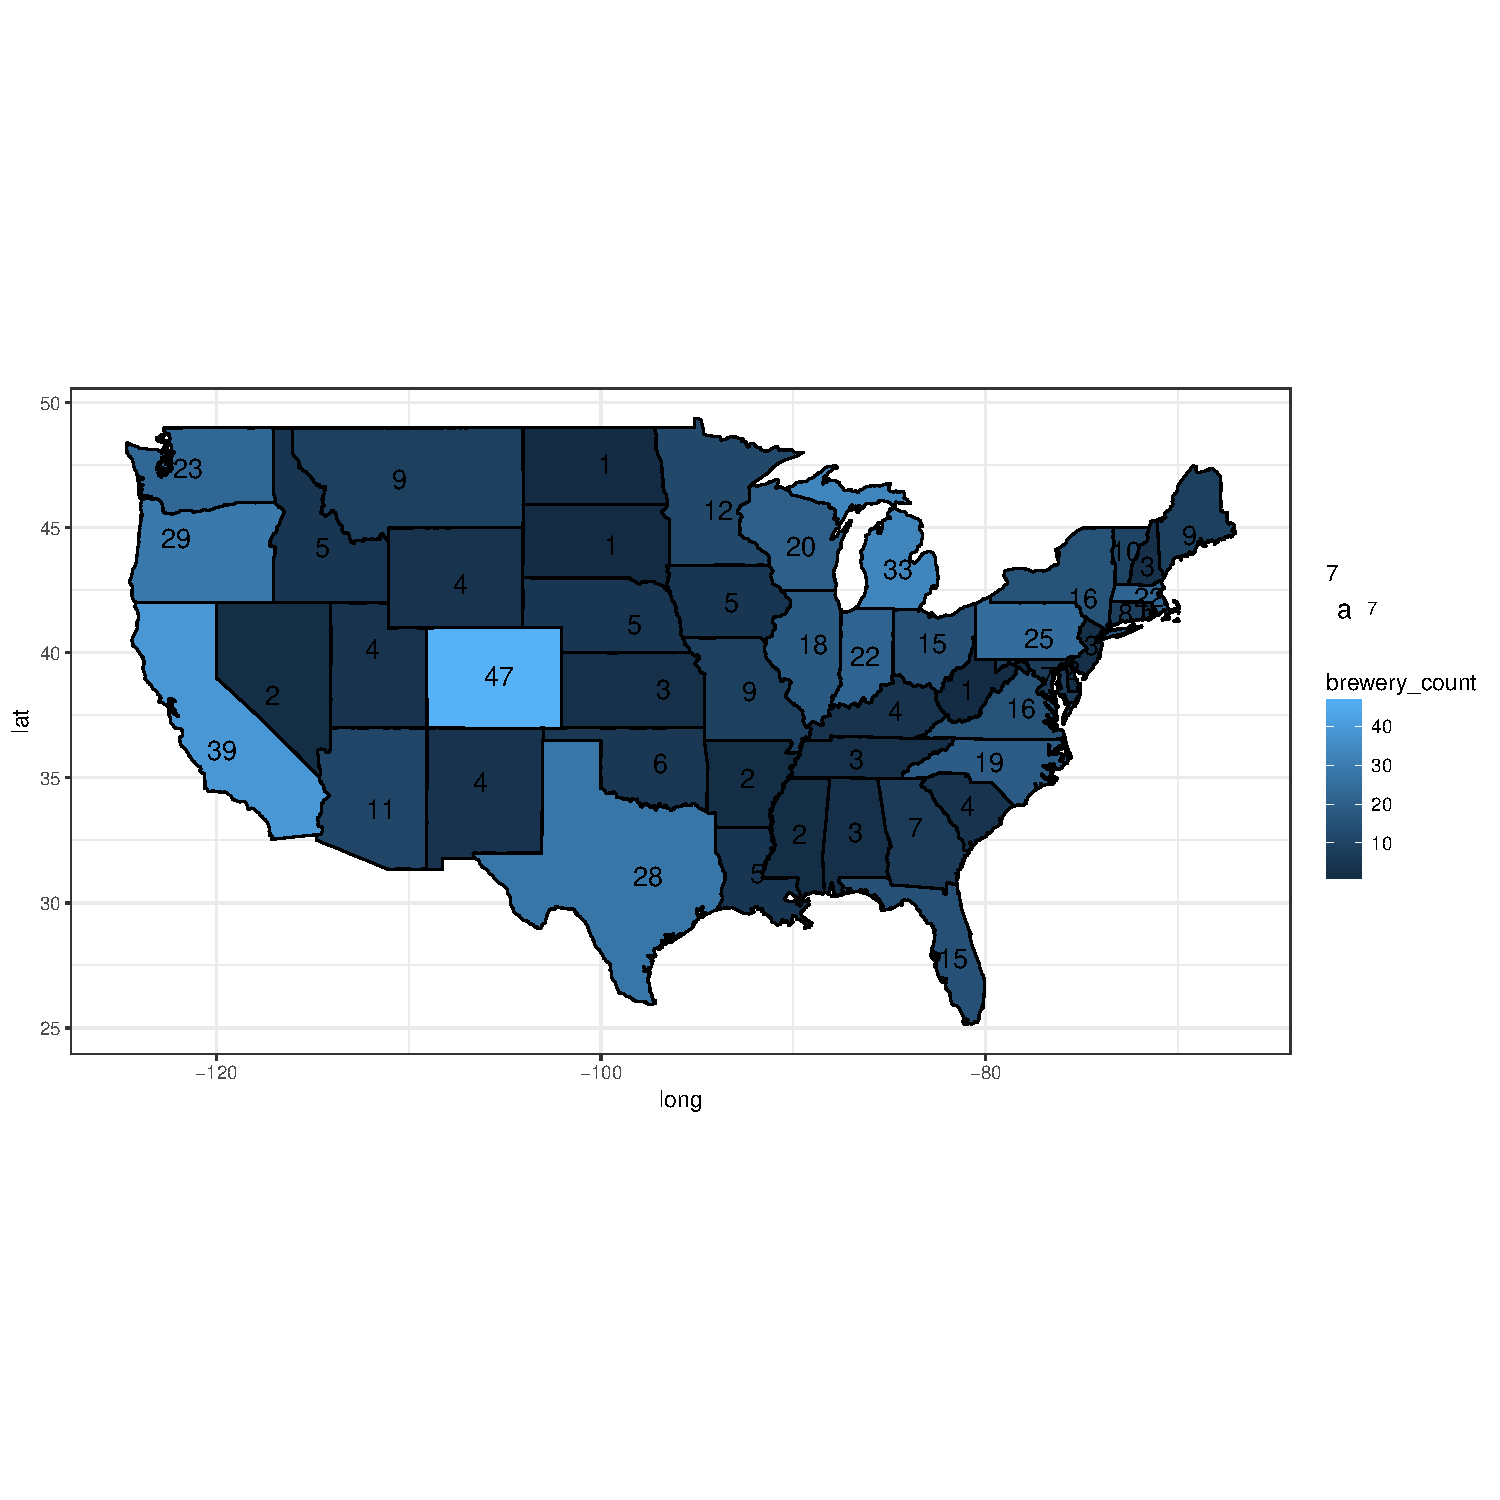
\includegraphics{Analysis_Final_files/figure-latex/unnamed-chunk-14-1.pdf}

\paragraph{QQ-Plot - Check for
Normality}\label{qq-plot---check-for-normality}

\begin{Shaded}
\begin{Highlighting}[]
\CommentTok{# QQ Plots of IBU and ABV}


\CommentTok{#calulate line fit}
\NormalTok{y <-}\StringTok{ }\KeywordTok{quantile}\NormalTok{((styles}\OperatorTok{$}\NormalTok{ibu }\OperatorTok\StringTok{ }\KeywordTok{na.omit}\NormalTok{()), }\KeywordTok{c}\NormalTok{(}\FloatTok{0.25}\NormalTok{, }\FloatTok{0.75}\NormalTok{))}
\NormalTok{x <-}\StringTok{ }\KeywordTok{qnorm}\NormalTok{(}\KeywordTok{c}\NormalTok{(}\FloatTok{0.25}\NormalTok{, }\FloatTok{0.75}\NormalTok{))}
\NormalTok{slope <-}\StringTok{ }\KeywordTok{diff}\NormalTok{(y)}\OperatorTok{/}\KeywordTok{diff}\NormalTok{(x)}
\NormalTok{y_int <-}\StringTok{ }\NormalTok{y[}\DecValTok{1}\NormalTok{] }\OperatorTok{-}\StringTok{ }\NormalTok{slope }\OperatorTok{*}\StringTok{ }\NormalTok{x[}\DecValTok{1}\NormalTok{]}

\NormalTok{qq_ibu <-}\StringTok{ }\KeywordTok{ggplot}\NormalTok{(styles, }\KeywordTok{aes}\NormalTok{(}\DataTypeTok{sample =}\NormalTok{ styles}\OperatorTok{$}\NormalTok{ibu)) }\OperatorTok{+}\StringTok{ }
\StringTok{              }\KeywordTok{geom_qq}\NormalTok{(}\DataTypeTok{shape =} \DecValTok{16}\NormalTok{, }\DataTypeTok{size =} \DecValTok{2}\NormalTok{, }\DataTypeTok{alpha =} \FloatTok{0.5}\NormalTok{) }\OperatorTok{+}
\StringTok{              }\KeywordTok{geom_abline}\NormalTok{(}\DataTypeTok{slope =}\NormalTok{ slope, }\DataTypeTok{intercept =}\NormalTok{ y_int, }\DataTypeTok{colour =}\StringTok{'red'}\NormalTok{, }\DataTypeTok{size =} \DecValTok{1}\NormalTok{) }\OperatorTok{+}
\StringTok{              }\KeywordTok{ggtitle}\NormalTok{(}\StringTok{"QQ-Plot of IBU"}\NormalTok{) }\OperatorTok{+}
\StringTok{              }\KeywordTok{theme_bw}\NormalTok{()  }\OperatorTok{+}
\StringTok{              }\KeywordTok{theme}\NormalTok{(}\DataTypeTok{plot.title =} \KeywordTok{element_text}\NormalTok{(}\DataTypeTok{hjust =} \FloatTok{0.5}\NormalTok{))}


\CommentTok{#calulate line fit}
\NormalTok{y <-}\StringTok{ }\KeywordTok{quantile}\NormalTok{((styles}\OperatorTok{$}\NormalTok{abv }\OperatorTok\StringTok{ }\KeywordTok{na.omit}\NormalTok{()), }\KeywordTok{c}\NormalTok{(}\FloatTok{0.25}\NormalTok{, }\FloatTok{0.75}\NormalTok{))}
\NormalTok{x <-}\StringTok{ }\KeywordTok{qnorm}\NormalTok{(}\KeywordTok{c}\NormalTok{(}\FloatTok{0.25}\NormalTok{, }\FloatTok{0.75}\NormalTok{))}
\NormalTok{slope <-}\StringTok{ }\KeywordTok{diff}\NormalTok{(y)}\OperatorTok{/}\KeywordTok{diff}\NormalTok{(x)}
\NormalTok{y_int <-}\StringTok{ }\NormalTok{y[}\DecValTok{1}\NormalTok{] }\OperatorTok{-}\StringTok{ }\NormalTok{slope }\OperatorTok{*}\StringTok{ }\NormalTok{x[}\DecValTok{1}\NormalTok{]  }

\NormalTok{qq_abv <-}\StringTok{ }\KeywordTok{ggplot}\NormalTok{(styles, }\KeywordTok{aes}\NormalTok{(}\DataTypeTok{sample =}\NormalTok{ styles}\OperatorTok{$}\NormalTok{abv)) }\OperatorTok{+}\StringTok{ }
\StringTok{            }\KeywordTok{geom_qq}\NormalTok{(}\DataTypeTok{shape =} \DecValTok{16}\NormalTok{, }\DataTypeTok{size =} \DecValTok{2}\NormalTok{, }\DataTypeTok{alpha =} \FloatTok{0.5}\NormalTok{) }\OperatorTok{+}
\StringTok{            }\KeywordTok{geom_abline}\NormalTok{(}\DataTypeTok{slope =}\NormalTok{ slope, }\DataTypeTok{intercept =}\NormalTok{ y_int, }\DataTypeTok{colour =}\StringTok{'red'}\NormalTok{, }\DataTypeTok{size =} \DecValTok{1}\NormalTok{) }\OperatorTok{+}
\StringTok{            }\KeywordTok{ggtitle}\NormalTok{(}\StringTok{"QQ-Plot of ABV"}\NormalTok{) }\OperatorTok{+}
\StringTok{            }\KeywordTok{theme_bw}\NormalTok{() }\OperatorTok{+}
\StringTok{            }\KeywordTok{theme}\NormalTok{(}\DataTypeTok{plot.title =} \KeywordTok{element_text}\NormalTok{(}\DataTypeTok{hjust =} \FloatTok{0.5}\NormalTok{))}


\KeywordTok{grid.arrange}\NormalTok{(qq_abv, qq_ibu)}
\end{Highlighting}
\end{Shaded}

\includegraphics{Analysis_Final_files/figure-latex/unnamed-chunk-15-1.pdf}

\paragraph{Histogram - Check for
Normality}\label{histogram---check-for-normality}

\begin{Shaded}
\begin{Highlighting}[]
\CommentTok{# Histograms of IBU and ABV}

\NormalTok{hist_ibu <-}\StringTok{ }\KeywordTok{ggplot}\NormalTok{(styles) }\OperatorTok{+}
\StringTok{              }\KeywordTok{geom_histogram}\NormalTok{(}\KeywordTok{aes}\NormalTok{(}\DataTypeTok{x=}\NormalTok{ibu)) }\OperatorTok{+}
\StringTok{              }\KeywordTok{theme}\NormalTok{(}\DataTypeTok{text =} \KeywordTok{element_text}\NormalTok{(}\DataTypeTok{size=}\DecValTok{10}\NormalTok{),}
                  \DataTypeTok{axis.text.x =} \KeywordTok{element_text}\NormalTok{(}\DataTypeTok{angle=}\DecValTok{90}\NormalTok{, }\DataTypeTok{hjust=}\DecValTok{1}\NormalTok{)) }

\NormalTok{hist_abv <-}\StringTok{ }\KeywordTok{ggplot}\NormalTok{(styles) }\OperatorTok{+}
\StringTok{              }\KeywordTok{geom_histogram}\NormalTok{(}\KeywordTok{aes}\NormalTok{(}\DataTypeTok{x=}\NormalTok{abv)) }\OperatorTok{+}
\StringTok{              }\KeywordTok{theme}\NormalTok{(}\DataTypeTok{text =} \KeywordTok{element_text}\NormalTok{(}\DataTypeTok{size=}\DecValTok{10}\NormalTok{),}
                  \DataTypeTok{axis.text.x =} \KeywordTok{element_text}\NormalTok{(}\DataTypeTok{angle=}\DecValTok{90}\NormalTok{, }\DataTypeTok{hjust=}\DecValTok{1}\NormalTok{)) }


\KeywordTok{grid.arrange}\NormalTok{(hist_abv, hist_ibu)}
\end{Highlighting}
\end{Shaded}

\begin{verbatim}
## `stat_bin()` using `bins = 30`. Pick better value with `binwidth`.
## `stat_bin()` using `bins = 30`. Pick better value with `binwidth`.
\end{verbatim}

\includegraphics{Analysis_Final_files/figure-latex/unnamed-chunk-16-1.pdf}

\paragraph{Boxplot - Check for
Outliers}\label{boxplot---check-for-outliers}

\begin{Shaded}
\begin{Highlighting}[]
\CommentTok{# Boxplots of IBU and ABV}


\NormalTok{ibu_outliers <-}\StringTok{ }\KeywordTok{boxplot}\NormalTok{(styles}\OperatorTok{$}\NormalTok{ibu, }\DataTypeTok{plot =} \OtherTok{FALSE}\NormalTok{)[[}\StringTok{"out"}\NormalTok{]]}

\NormalTok{abv_outliers <-}\StringTok{ }\KeywordTok{boxplot}\NormalTok{(styles}\OperatorTok{$}\NormalTok{abv, }\DataTypeTok{plot =} \OtherTok{FALSE}\NormalTok{)[[}\StringTok{"out"}\NormalTok{]]}


\NormalTok{x<-}\KeywordTok{boxplot}\NormalTok{(styles}\OperatorTok{$}\NormalTok{ibu, }\DataTypeTok{plot =} \OtherTok{FALSE}\NormalTok{)}

\NormalTok{bp_abv <-}\StringTok{ }\KeywordTok{ggplot}\NormalTok{((styles }\OperatorTok\StringTok{ }\KeywordTok{drop_na}\NormalTok{(abv)), }\KeywordTok{aes}\NormalTok{(}\DataTypeTok{x=}\StringTok{""}\NormalTok{, }\DataTypeTok{y=}\NormalTok{abv)) }\OperatorTok{+}
\StringTok{      }\KeywordTok{geom_point}\NormalTok{(}\KeywordTok{aes}\NormalTok{(}\DataTypeTok{fill =} \KeywordTok{ifelse}\NormalTok{((abv }\OperatorTok\StringTok{ }\NormalTok{abv_outliers),}\StringTok{"Outlier"}\NormalTok{,}\StringTok{"Valid"}\NormalTok{)), }
                 \DataTypeTok{size =} \DecValTok{4}\NormalTok{, }
                 \DataTypeTok{shape =} \DecValTok{21}\NormalTok{, }
                 \DataTypeTok{position =} \KeywordTok{position_jitter}\NormalTok{())}\OperatorTok{+}
\StringTok{      }\KeywordTok{stat_boxplot}\NormalTok{(}\DataTypeTok{geom =}\StringTok{'errorbar'}\NormalTok{) }\OperatorTok{+}
\StringTok{      }\KeywordTok{geom_boxplot}\NormalTok{(}\DataTypeTok{alpha=}\NormalTok{.}\DecValTok{5}\NormalTok{, }
                   \DataTypeTok{outlier.shape =} \OtherTok{NA}\NormalTok{) }\OperatorTok{+}
\StringTok{      }\KeywordTok{guides}\NormalTok{(}\DataTypeTok{fill=}\KeywordTok{guide_legend}\NormalTok{(}\DataTypeTok{title=} \OtherTok{NULL}\NormalTok{)) }\OperatorTok{+}
\StringTok{      }\KeywordTok{xlab}\NormalTok{(}\StringTok{"Beer Styles"}\NormalTok{) }\OperatorTok{+}
\StringTok{      }\KeywordTok{ylab}\NormalTok{(}\StringTok{"Alcohol by Volume (ABV)"}\NormalTok{) }\OperatorTok{+}
\StringTok{      }\KeywordTok{scale_y_continuous}\NormalTok{(}\DataTypeTok{position =} \StringTok{"right"}\NormalTok{, }
                         \DataTypeTok{breaks =} \KeywordTok{c}\NormalTok{(.}\DecValTok{025}\NormalTok{, .}\DecValTok{05}\NormalTok{, .}\DecValTok{075}\NormalTok{, .}\DecValTok{1}\NormalTok{, .}\DecValTok{125}\NormalTok{), }
                         \DataTypeTok{limits =} \KeywordTok{c}\NormalTok{(}\FloatTok{0.025}\NormalTok{, .}\DecValTok{125}\NormalTok{)) }\OperatorTok{+}
\StringTok{      }\KeywordTok{coord_flip}\NormalTok{()}


\NormalTok{bp_ibu <-}\StringTok{ }\KeywordTok{ggplot}\NormalTok{((styles }\OperatorTok\StringTok{ }\KeywordTok{drop_na}\NormalTok{(ibu)), }\KeywordTok{aes}\NormalTok{(}\DataTypeTok{x=}\StringTok{""}\NormalTok{, }\DataTypeTok{y=}\NormalTok{ibu)) }\OperatorTok{+}
\StringTok{      }\KeywordTok{geom_point}\NormalTok{(}\KeywordTok{aes}\NormalTok{(}\DataTypeTok{fill =} \KeywordTok{ifelse}\NormalTok{((ibu }\OperatorTok\StringTok{ }\NormalTok{ibu_outliers),}\StringTok{"Outlier"}\NormalTok{,}\StringTok{"Valid"}\NormalTok{)),}
                 \DataTypeTok{size =} \DecValTok{4}\NormalTok{, }
                 \DataTypeTok{shape =} \DecValTok{21}\NormalTok{, }
                 \DataTypeTok{position =} \KeywordTok{position_jitter}\NormalTok{())}\OperatorTok{+}
\StringTok{      }\KeywordTok{stat_boxplot}\NormalTok{(}\DataTypeTok{geom =}\StringTok{'errorbar'}\NormalTok{) }\OperatorTok{+}
\StringTok{      }\KeywordTok{geom_boxplot}\NormalTok{(}\DataTypeTok{alpha =}\NormalTok{ .}\DecValTok{75}\NormalTok{, }
                   \DataTypeTok{outlier.shape =} \OtherTok{NA}\NormalTok{) }\OperatorTok{+}
\StringTok{      }\KeywordTok{guides}\NormalTok{(}\DataTypeTok{fill=}\KeywordTok{guide_legend}\NormalTok{(}\DataTypeTok{title=} \OtherTok{NULL}\NormalTok{)) }\OperatorTok{+}
\StringTok{      }\KeywordTok{xlab}\NormalTok{(}\StringTok{"Beer Styles"}\NormalTok{) }\OperatorTok{+}
\StringTok{      }\KeywordTok{ylab}\NormalTok{(}\StringTok{"International Bitterness Units (IBU)"}\NormalTok{) }\OperatorTok{+}
\StringTok{      }\KeywordTok{scale_y_continuous}\NormalTok{(}\DataTypeTok{breaks =} \KeywordTok{c}\NormalTok{(}\DecValTok{0}\NormalTok{, }\DecValTok{25}\NormalTok{, }\DecValTok{50}\NormalTok{, }\DecValTok{75}\NormalTok{, }\DecValTok{100}\NormalTok{, }\DecValTok{125}\NormalTok{, }\DecValTok{150}\NormalTok{), }
                         \DataTypeTok{limits =} \KeywordTok{c}\NormalTok{(}\DecValTok{0}\NormalTok{, }\DecValTok{150}\NormalTok{)) }\OperatorTok{+}
\StringTok{      }\KeywordTok{coord_flip}\NormalTok{()}

\KeywordTok{grid.arrange}\NormalTok{(bp_abv, bp_ibu)}
\end{Highlighting}
\end{Shaded}

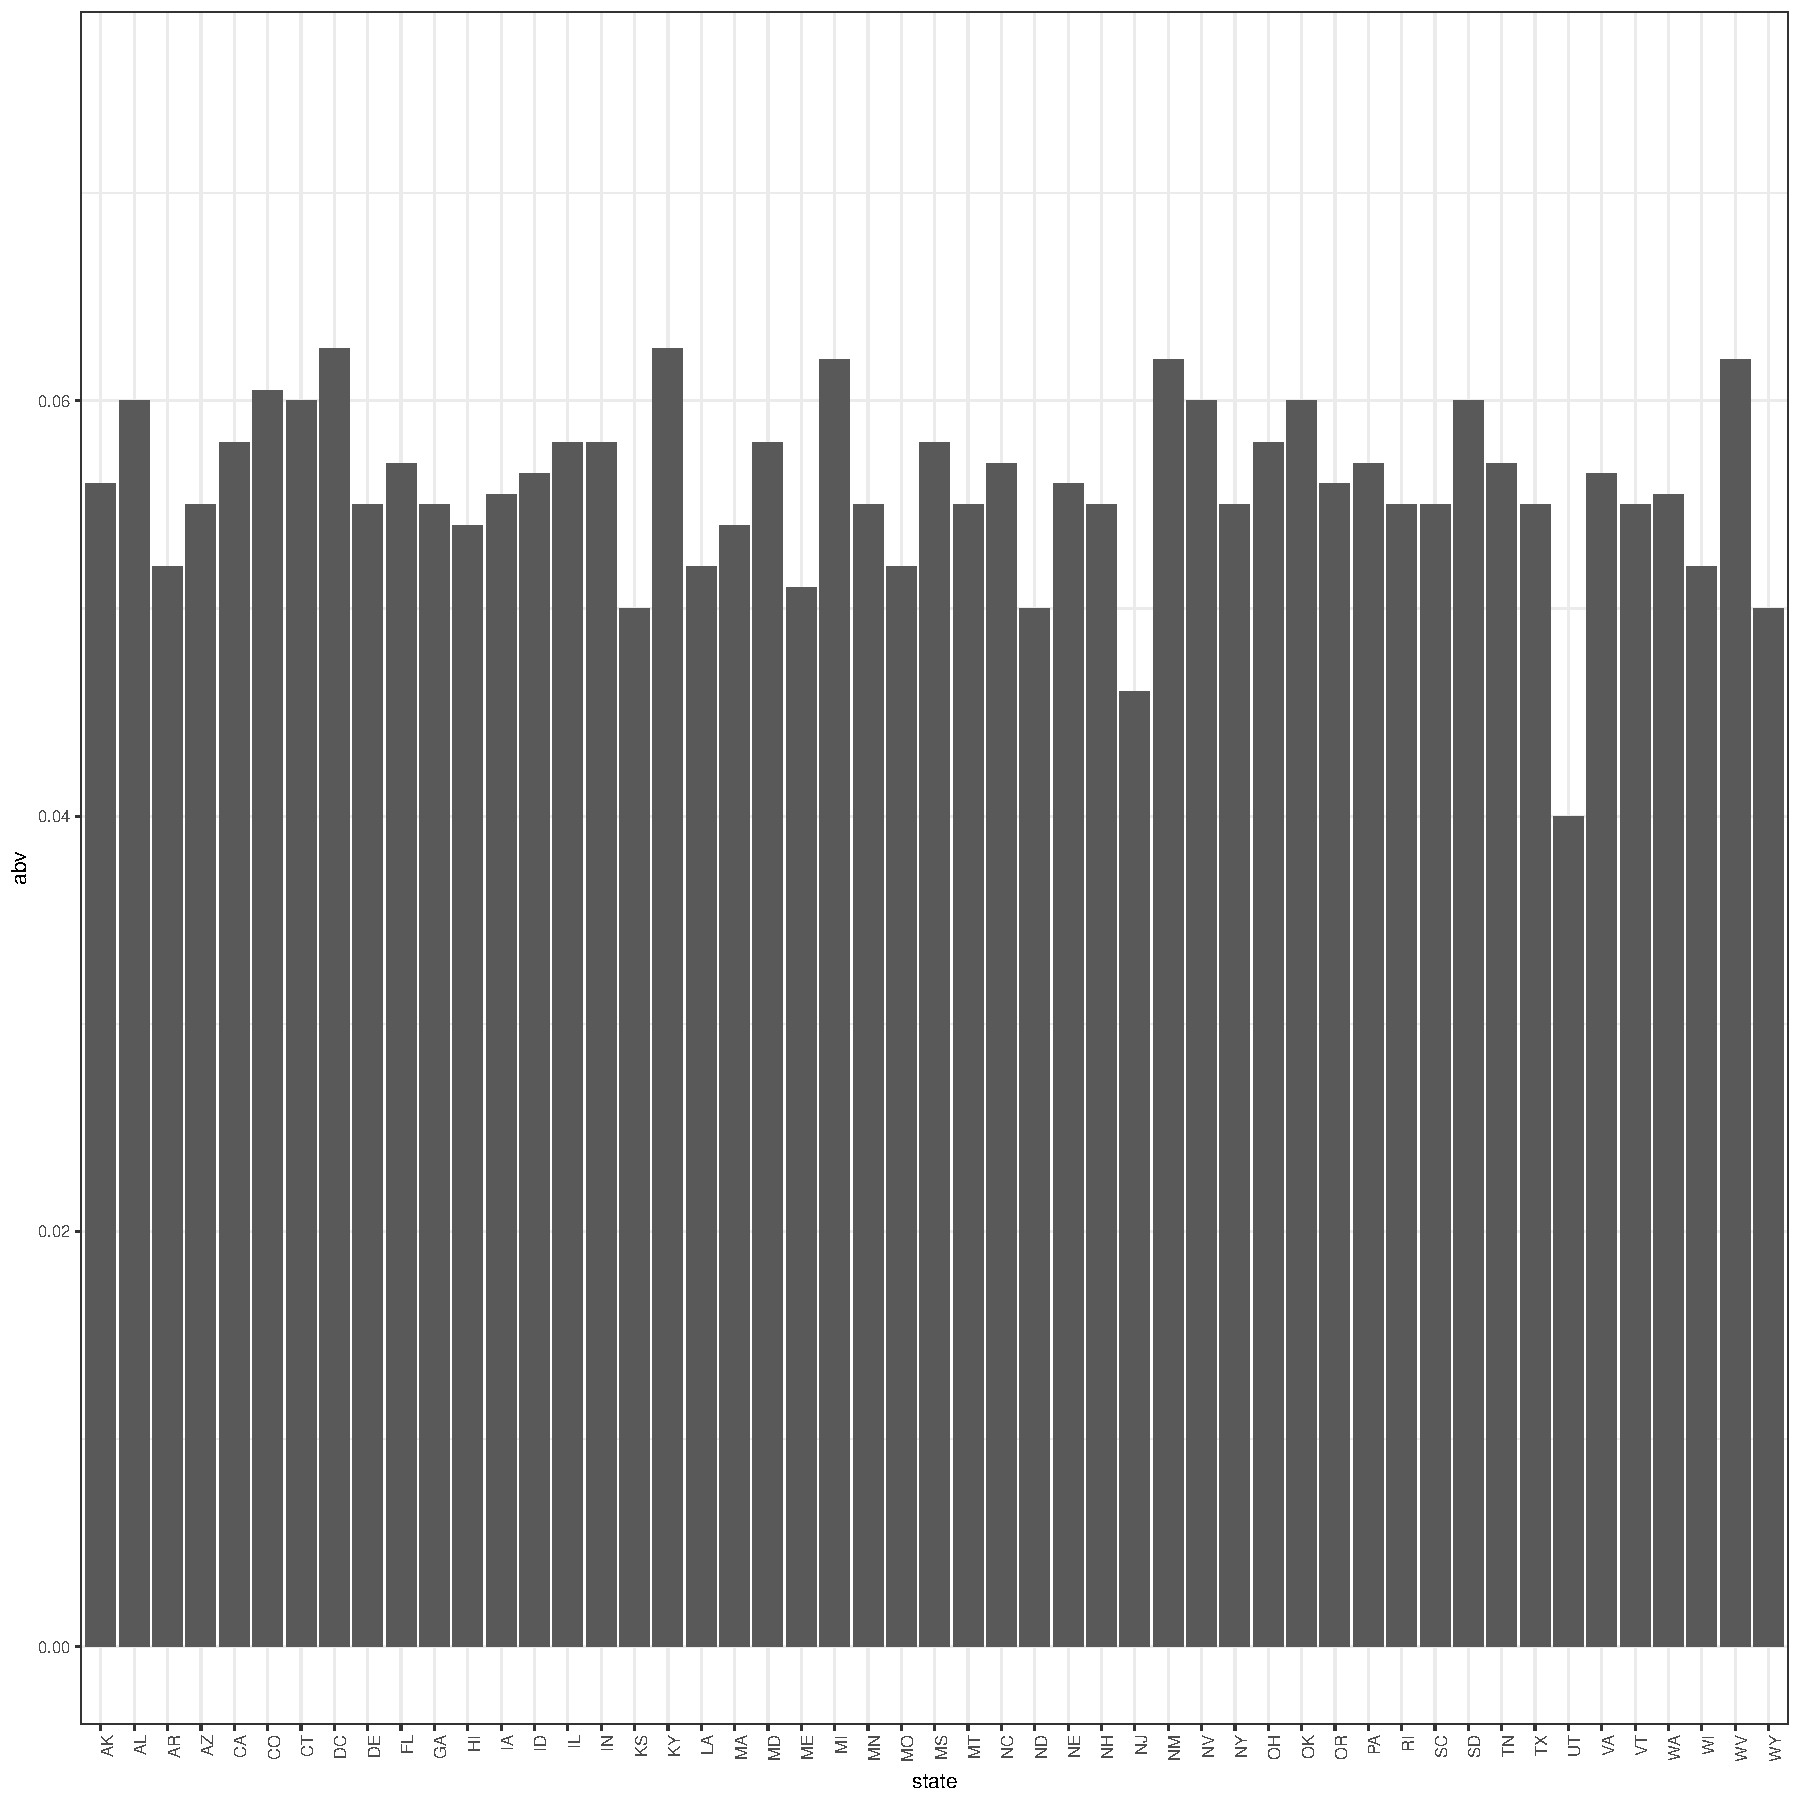
\includegraphics{Analysis_Final_files/figure-latex/unnamed-chunk-17-1.pdf}

\begin{itemize}
\tightlist
\item
  Due to the lack of normality of the IBU variable and the presence of
  outliers in both variables, we will use the Spearman Rank-Correlation
  test as an alternative to the preferred Pearson Correlation.
\end{itemize}

\paragraph{Spearman Rank-Order
Correlation}\label{spearman-rank-order-correlation}

\begin{verbatim}
+ More info on Spearman test: https://statistics.laerd.com/statistical-guides/spearmans-rank-order-correlation-statistical-guide.php
\end{verbatim}

\begin{itemize}
\tightlist
\item
  Hypotheses:

  \begin{itemize}
  \tightlist
  \item
    H\textsubscript{o}: \(\rho = 0\)
  \item
    H\textsubscript{A}: \(\rho \neq 0\)
  \end{itemize}
\end{itemize}

\begin{Shaded}
\begin{Highlighting}[]
\CommentTok{# Significance test}
\NormalTok{spear_test_result <-}\StringTok{ }\KeywordTok{cor.test}\NormalTok{(styles}\OperatorTok{$}\NormalTok{ibu, styles}\OperatorTok{$}\NormalTok{abv, }\DataTypeTok{method =} \StringTok{"spearman"}\NormalTok{, }\DataTypeTok{conf.level =}\NormalTok{ .}\DecValTok{05}\NormalTok{, }\DataTypeTok{exact=}\OtherTok{FALSE}\NormalTok{)}

\NormalTok{spear_test_result}
\end{Highlighting}
\end{Shaded}

\begin{verbatim}
Spearman's rank correlation rho
\end{verbatim}

data: styles\(ibu and styles\)abv S = 153570000, p-value \textless{}
2.2e-16 alternative hypothesis: true rho is not equal to 0 sample
estimates: rho 0.6677798

\begin{Shaded}
\begin{Highlighting}[]
\NormalTok{r_sq <-}\StringTok{ }\NormalTok{spear_test_result[[}\StringTok{"estimate"}\NormalTok{]][[}\StringTok{"rho"}\NormalTok{]]}\OperatorTok{^}\DecValTok{2} \CommentTok{# capture r-squared}

\NormalTok{r_sq}
\end{Highlighting}
\end{Shaded}

{[}1{]} 0.4459299

\paragraph{Conclusion}\label{conclusion}

There is strong evidence that the ABV and IBU are positively associated
(p-value \textless{} 0.001 from a Spearman Rank-Order Correlation). At a
95\% confidence level, the IBU rating accounts for 44.5\% of the
variation in the ABV . While IBU and ABV certainly have a correlation,
the correlation is weak (\(r^2 = 0.445\)). Thus, we reject the null
hypothesis that IBU rating and ABV are un-corrolated across the beer
styles in our sample. Beer styles were not randomly assigned to any
treatment and we do not know if the beer data were randomly selected, so
we must limit our results to indicating an association between IBU
rating an ABV. No causality or inferences to larger populations can be
drawn.

\subsection{Write datasets to file}\label{write-datasets-to-file}

\begin{Shaded}
\begin{Highlighting}[]
\KeywordTok{write.csv}\NormalTok{( beer_clean,}\DataTypeTok{file =} \StringTok{'../data/beer_clean.csv'}\NormalTok{, }\DataTypeTok{row.names =} \OtherTok{FALSE}\NormalTok{)}
\KeywordTok{write.csv}\NormalTok{( breweries_clean,}\DataTypeTok{file =} \StringTok{'../data/breweries_clean.csv'}\NormalTok{, }\DataTypeTok{row.names =} \OtherTok{FALSE}\NormalTok{)}
\end{Highlighting}
\end{Shaded}

\subsection{Appendex}\label{appendex}

\paragraph{Session Info}\label{session-info}

\begin{Shaded}
\begin{Highlighting}[]
\KeywordTok{sessionInfo}\NormalTok{()}
\end{Highlighting}
\end{Shaded}

R version 3.5.0 (2018-04-23) Platform: x86\_64-w64-mingw32/x64 (64-bit)
Running under: Windows 10 x64 (build 16299)

Matrix products: default

locale: {[}1{]} LC\_COLLATE=English\_United States.1252 {[}2{]}
LC\_CTYPE=English\_United States.1252\\
{[}3{]} LC\_MONETARY=English\_United States.1252 {[}4{]} LC\_NUMERIC=C\\
{[}5{]} LC\_TIME=English\_United States.1252

attached base packages: {[}1{]} stats graphics grDevices utils datasets
methods base

other attached packages: {[}1{]} bindrcpp\_0.2.2 gridExtra\_2.3
magrittr\_1.5\\
{[}4{]} summarytools\_0.8.5 RColorBrewer\_1.1-2 maps\_3.3.0\\
{[}7{]} ggplot2\_2.2.1 knitr\_1.20 tidyr\_0.8.1\\
{[}10{]} dplyr\_0.7.5

loaded via a namespace (and not attached): {[}1{]} Rcpp\_0.12.17
highr\_0.7 pillar\_1.2.3\\
{[}4{]} compiler\_3.5.0 pryr\_0.1.4 plyr\_1.8.4\\
{[}7{]} bindr\_0.1.1 bitops\_1.0-6 tools\_3.5.0\\
{[}10{]} digest\_0.6.15 lubridate\_1.7.4 evaluate\_0.10.1\\
{[}13{]} tibble\_1.4.2 gtable\_0.2.0 pkgconfig\_2.0.1\\
{[}16{]} rlang\_0.2.1 cli\_1.0.0 yaml\_2.1.19\\
{[}19{]} stringr\_1.3.1 rprojroot\_1.3-2 grid\_3.5.0\\
{[}22{]} tidyselect\_0.2.4 glue\_1.2.0 R6\_2.2.2\\
{[}25{]} rmarkdown\_1.10 pander\_0.6.1 purrr\_0.2.5\\
{[}28{]} rapportools\_1.0 backports\_1.1.2 scales\_0.5.0\\
{[}31{]} codetools\_0.2-15 htmltools\_0.3.6 matrixStats\_0.53.1 {[}34{]}
assertthat\_0.2.0 colorspace\_1.3-2 labeling\_0.3\\
{[}37{]} utf8\_1.1.4 stringi\_1.1.7 RCurl\_1.95-4.10\\
{[}40{]} lazyeval\_0.2.1 munsell\_0.5.0 crayon\_1.3.4


\end{document}
